\chapter{Implementacja sprzętowa systemu wizyjnego}
\section{Układy FPGA}
Najważniejszym i najbardziej czasochłonnym elementem pracy była implementacja algorytmu śledzącego na obiekcie latającym. Obecnie istnieje możliwość skorzystania z przeróżnych cyfrowych jednostek obliczeniowych, które dzieli się, jak przedstawiono poniżej:
\begin{itemize}
	\item brak możliwości zmiany funkcjonalności po wyprodukowaniu układu:
	\begin{itemize}
		\item procesory ASIP (ang. \textit{Application Specific Instruction Set Processor}) - zaprojektowane z dedykowanym zestawem instrukcji		
		\item układy ASIC (ang. \textit{Application Specific Integrated Circuit}) - zaprojektowane do realizacji określonej z góry zadań
		\item procesory ogólnego przeznaczenia CPU (ang. \textit{Central Processing Unit})
		\item procesory graficzne GPU (ang. \textit{Graphics Processing Unit})
		\item procesory sygnałowe DSP (ang. \textit{Digital Signal Processor})
	\end{itemize}
	\item z możliwością konfiguracji po procesie produkcyjnym:
	\begin{itemize} 
		\item układy rekonfigurowalne z architekturą gruboziarnistą
		\item układy rekonfigurowalne z architekturą drobnoziarnistą - FPGA (ang. \textit{Field-Programmable Gate Array}) oraz CPLD (ang. \textit{Complex Programmable Logic Device})
	\end{itemize}
\end{itemize}
Układy ASIC są niestety drogie w prototypowaniu. Procesory CPU nie pozwolą na przetworzenie tak wielkiej ilości danych w czasie rzeczywistym. Z kolei druga grupa urządzeń ma atut polegający na możliwości zmiany architektury układu oraz zrównoleglenia obliczeń tak bardzo, jak tylko pozwala na to ilość dostępnych zasobów. Dodatkowo - i paradoksalnie zarazem - urządzenia te charakteryzują się stosunkowo niskim zapotrzebowaniem na energię. Ma to istotne znaczenie, mając na uwadze światowy trend poszukiwań energooszczędnych rozwiązań w każdej branży. Obszary, w których FPGA znajduje zastosowanie to między innymi:
\begin{itemize}
	\item studia dźwiękowe,
	\item telekomunikacja,
	\item przemysł motoryzacyjny/zbrojeniowy/lotniczy/kosmiczny,
	\item szyfrowanie i przetwarzanie danych,
	\item aparatura medyczna,
	\item systemy wizyjne.
\end{itemize}
To wszystko nie oznacza jednak, że układy FPGA nie są pozbawione wad. Przykładowo, nie można zrealizować na nich niektórych rodzajów algorytmów, głównie rekurencyjnych. Ponadto, sam proces rozwoju konkretnej architektury nie należy do najprostszych i może wymagać potwierdzenia funkcjonalności na kilka sposobów:
\begin{itemize}
	\item porównanie wyników z innym, konwencjonalnym środowiskiem (MATLAB, OpenCV),
	\item symulacja projektu HDL na komputerze,
	\item weryfikacja wybranych sygnałów na układzie przy użyciu zintegrowanego analizatora logicznego (SignalTap dla urządzeń Altery, ILA dla układów Xilinxa).
\end{itemize}
Część problemów bywa z czasem rozwiązywana przez producentów. Stopień skomplikowania projektu można znacznie zredukować, wykorzystując dostępną z oprogramowaniem własność intelektualną - odpowiednio skonfigurowane tzw. IP Core'y - i łącząc sygnały pomiędzy nimi na graficznych diagramach. Co więcej, narzędzie Vivado High-Level Synthesis (HLS) oferuje możliwość adaptacji języka C/C++ do technologii FPGA, upraszczając proces powstawania architektury. \newline Postępująca zwłaszcza w ostatnich latach integracja i zmniejszanie procesu technologicznego pozwoliły na stworzenie układów łączących logikę programowalną (FPGA) oraz dwurdzeniowy procesor ARM. Krzem, na którym oprócz jednostki obliczeniowej znajdują się różne peryferia, nosi nazwę układu heterogenicznego, w branży bardziej znanego jako \textit{System on a Chip} (SoC). Dzięki magistrali (przykładowo AXI) zapewniającej szybką wymianę danych pomiędzy blokami, taki układ pozwala łączyć możliwość zrównoleglania obliczeń, którą daje logika programowalna (\textit{ang. PL - Programmable Logic}), oraz prostotę rozwoju oprogramowania uruchamianego na procesorze (\textit{ang. PS - Processing System}). W tej ostatniej części istnieje możliwość uruchomienia systemu operacyjnego (jednej ze specjalnych dystrybucji Linuxowych) lub nawet stworzenia konfiguracji opartej o wieloprocesorowość asynchroniczną (ang. AMP). Warto tu zauważyć, że narzędzia syntezy logiki od dawna oferowały możliwość stworzenia softprocesorów w układach FPGA (Altera - Nios, Xilinx - MicroBlaze), jednak te rozwiązania istotnie ograniczały dostępne zasoby, a częstotliwość taktowania takich komponentów rzadko przekraczała 200 MHz. \newline

Powyższa charakterystyka przekonuje, że układy FPGA, a zwłaszcza SoC mógłby być szczególnie doceniony na platformie latającej, gdyż byłby w stanie sprostać wymaganiom stawianym przez zadanie przetwarzania obrazu w czasie rzeczywistym, a dzięki niewielkim wymiarom i niskiemu zużyciu energii nie stanowiłby wielkiego obciążenia przy i tak już mocno ograniczonym czasie lotu na jednej baterii. \newline
Ze względu na charakter pracy użyto w niej układu ZYNQ SoC firmy Xilinx. Oczywiście, ze względu na poziom skomplikowania montażu tego urządzenia nie podjęto decyzji o prototypowaniu własnego obwodu drukowanego, lecz wykorzystano niewielki, lecz bogaty w peryferia zestaw PYNQ z układem ZYNQ SoC XC7Z020. Oprogramowaniem wspierającym rozwój architektury na to urządzenie jest pakiet Xilinx Vivado + SDK.

\section{Tor wizyjny w układzie FPGA}
\label{sec:counter}
Stworzony system wizyjny jest złożonym drzewem zależności pomiędzy wieloma modułami. By jednak był on torem wizyjnym, konieczne jest odebranie sygnału wideo z zewnątrz - w tym wypadku poprzez port HDMI - i poprawne zdekodowanie go do podstawowej, użytecznej przestrzeni barw RGB. Taki zestaw sygnałów jest dość prosty do uwzględnienia w tworzonych algorytmach. Opcjonalne i zalecane jest również wyprowadzenie przetworzonego sygnału RGB na monitor, który pozwoli zweryfikować poprawność tworzonej architektury. Wyżej opisany szkielet został stworzony w tzw. Block Designie, a poza modułami firmy Xilinx wykorzystano konwertery DVI$\rightarrow$RGB oraz RGB$\rightarrow$DVI dostarczone przez firmę Digilent - producenta zestawu PYNQ. Dodatkowo, podstawowym źródłem taktowania został dostarczany z karty PYNQ zegar o częstotliwości $125$MHz oraz sygnał inicjujący działanie algorytmu, pochodzący z odbiornika radiowego.

 

Sygnały wideo, które można wyodrębnić po zdekodowaniu, to:
\begin{itemize}
	\item zegar taktujący pikseli ($74.25$MHz)
	\item kolor czerwony R (8 bitów),
	\item kolor zielony G (8 bitów),
	\item kolor niebieski B (8 bitów),
	\item synchronizacja pozioma - poziom wysoki sygnalizuje koniec poziomej linii,
	\item synchronizacja pionowa - poziom wysoki sygnalizuje koniec klatki obrazu,
	\item sygnał aktywny - poziom wysoki sygnalizuje obecność poprawnego piksela.
\end{itemize}
Z góry założono, że transmisja i przetwarzanie wideo będzie się odbywać w oparciu o standard \textit{720p/60fps}. Uwzględniając narzut dany przez sygnały sterujące, ostateczna częstotliwość taktowania piksela wynosi w tym przypadku $74.25$MHz. To właśnie ten zegar, nazywany dalej w pracy \textit{\boldmath pixel\char`_clk}, stanowi podstawę potokowego przetwarzania obrazów w układzie FPGA. Poniższa ilustracja przedstawia zapis klatki z sygnałami sterującymi, gdzie jednostką jest cykl zegara taktującego piksel. 

\begin{figure}[h]
	\centering
	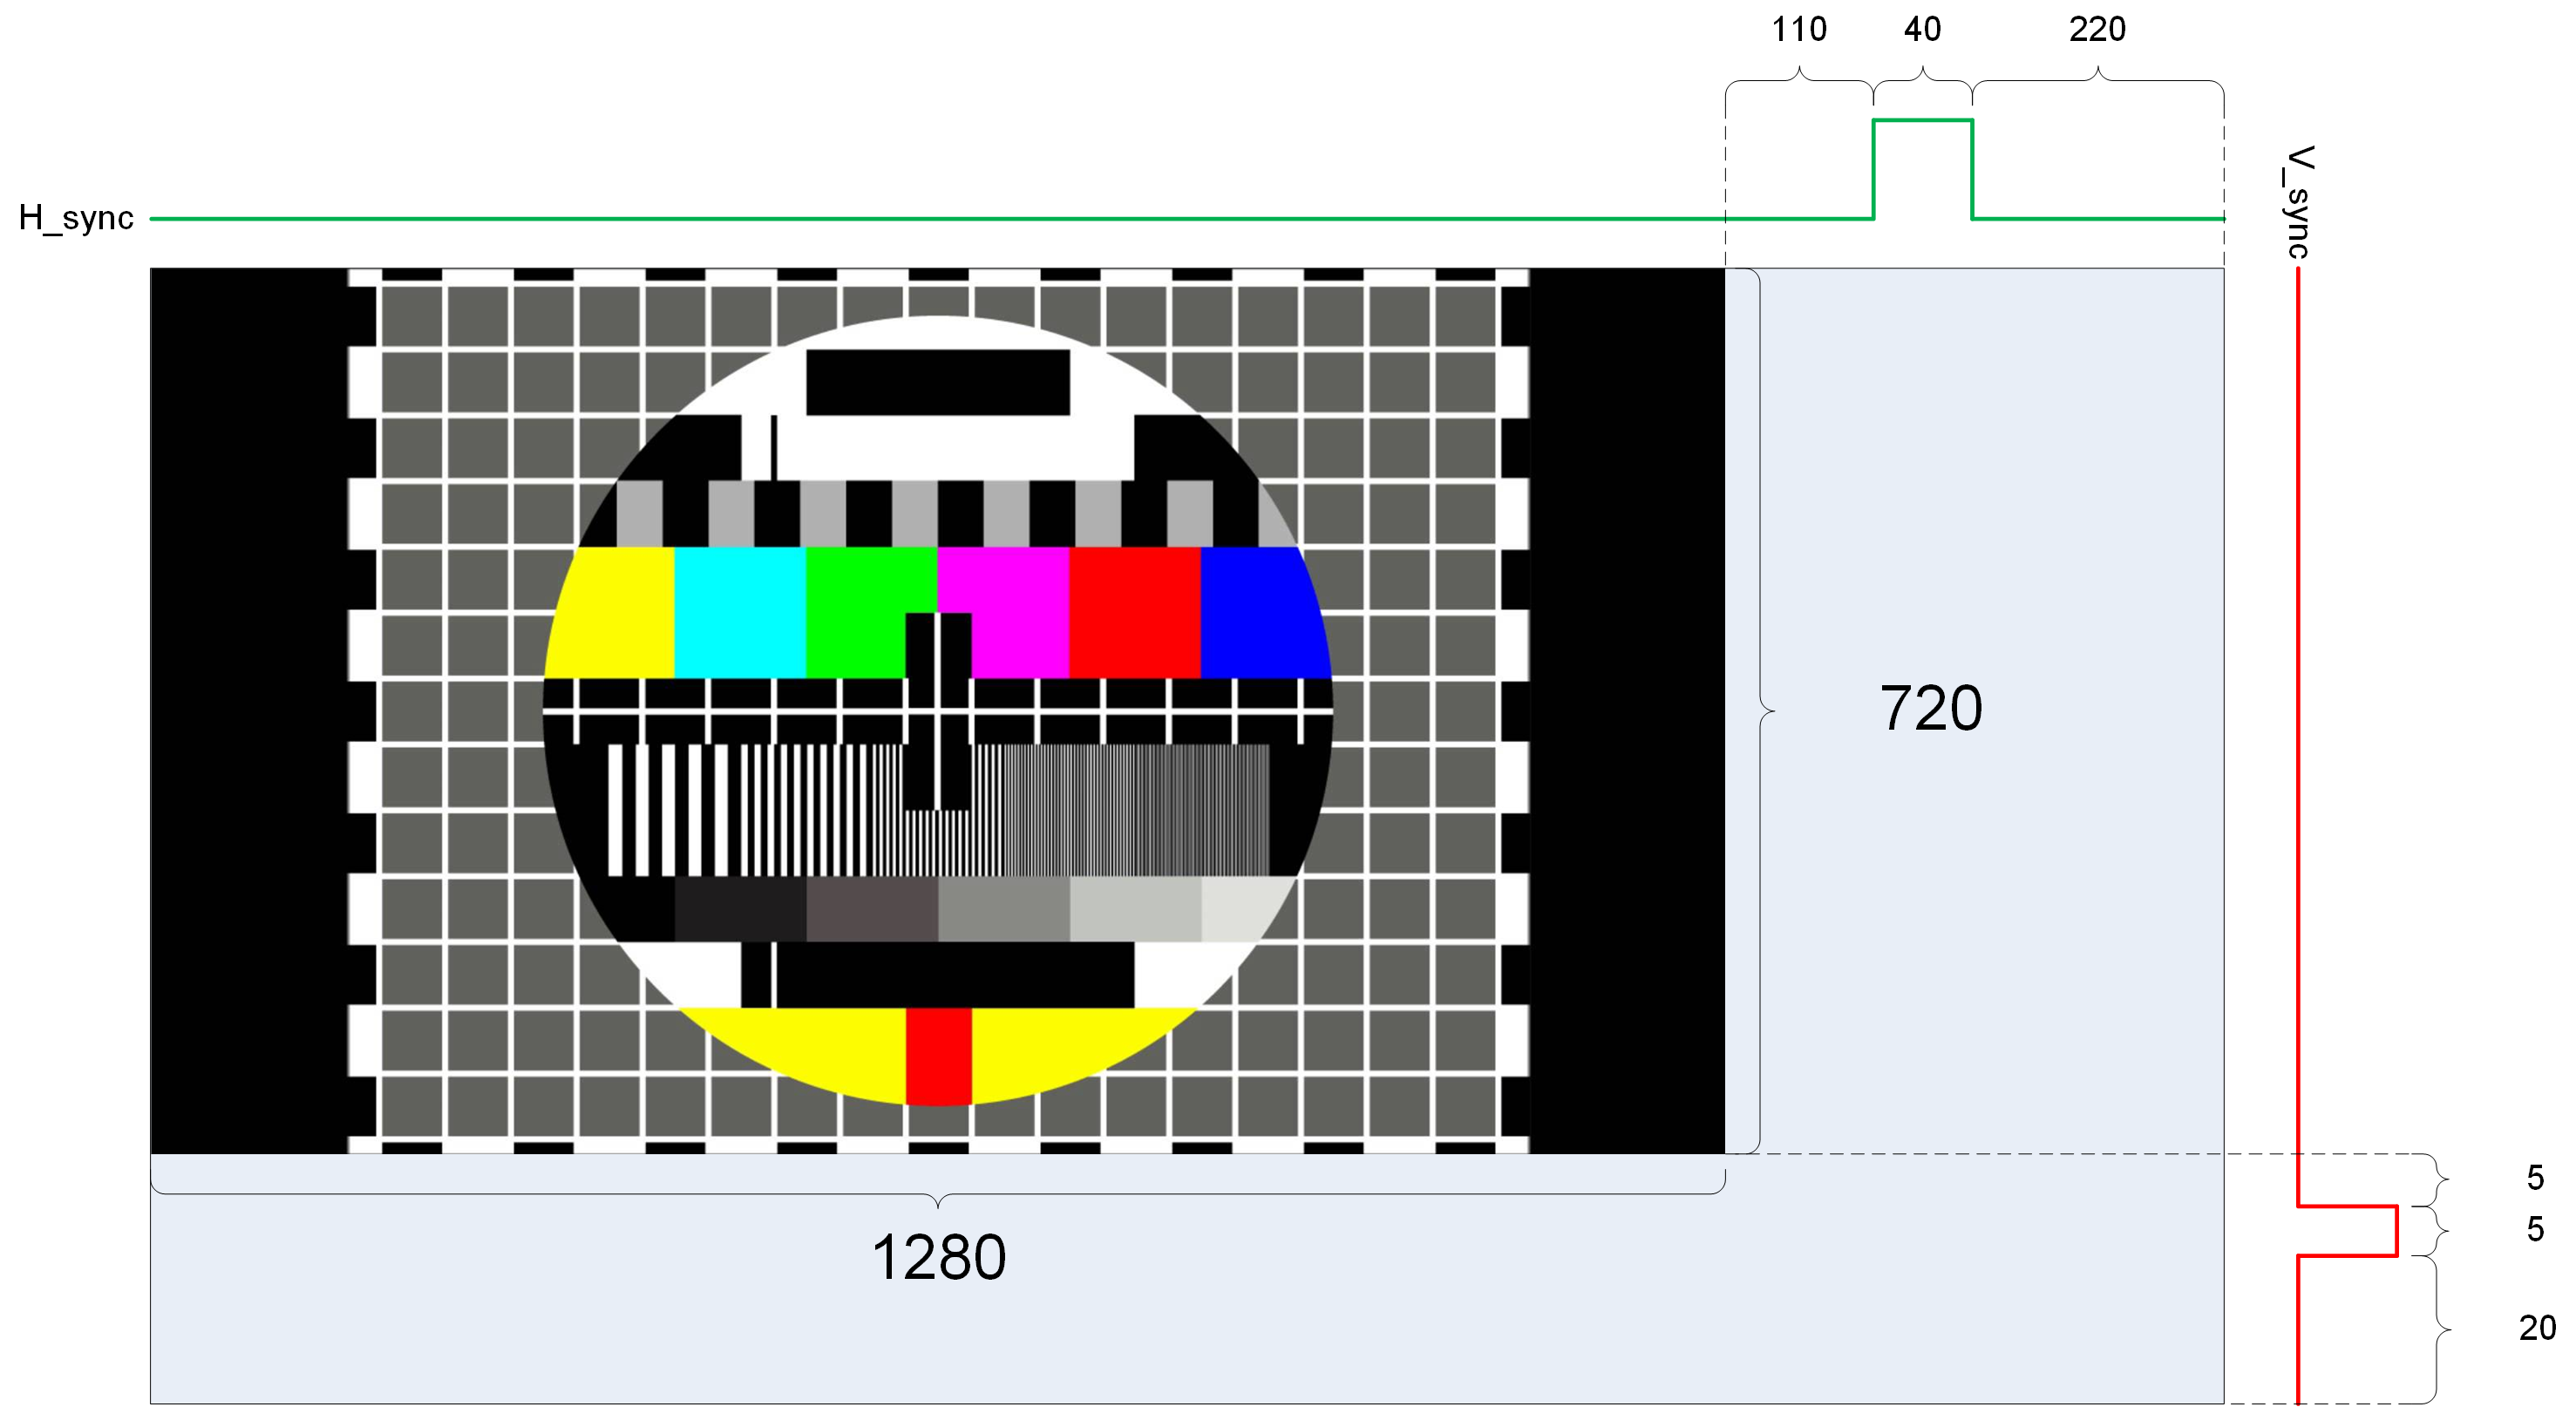
\includegraphics[width=17cm]{4_720p.png}
	\caption{Schemat zapisu klatki w rozdzielczości $720p$}
	\label{fig:720_frame}
\end{figure}

Algorytmy opisane w dalszej części pracy będą często posiłkować się informacją o aktualnym położeniu piksela na właściwym obrazie. Stworzono w tym celu licznik kalkulujący tę pozycję dla osi pionowej i poziomej w oparciu o długości trwania sygnałów kontrolnych z rysunku \ref{fig:720_frame}. 

 
\section{Realizacja algorytmu MeanShift}
Bazą do pracy nad implementacją było określenie wielkości obszaru śledzonego. Uwzględniając parametry optyczne kamery, jak i rozdzielczość wejściową materiału wideo podjęto decyzję o śledzeniu obszaru o wymiarach $100 \times 100$ pikseli. Analizując możliwości pracy układu okazało się, że algorytm jest w stanie przetwarzać każdą otrzymaną klatkę (lub raczej jej określony fragment) - częstotliwość jego pracy wynosi zatem \textit{60Hz}.\newline
Wstępnym etapem na drodze danych w algorytmie MeanShift jest konwersja przestrzeni barw, realizowana zgodnie ze wzorami \ref{HSV_first}-\ref{HSV_last} w module \textit{rgb2hsv}. Moduł działa w trybie potokowym pracując na zegarze \textit{pixel\char`_clk} i odpowiednio opóźnia wszystkie sygnały sterujące, co jest istotnym warunkiem poprawnego rozpoznawania odpowiednich pikseli w dalszych etapach przetwarzania.
Dane te są na bieżąco dostarczane do modułu \textit{Meanshift}, realizującego główną część zadań. 

\subsection{Inicjalizacja}
Mimo, że właściwe działanie algorytmu ma miejsce po otrzymaniu sygnału zewnętrznego (\textit{algorithm\char`_en}), wymaga on wcześniejszej inicjalizacji - odbywa się ona tuż po zaprogramowaniu układu FPGA. W głównej mierze jest ona związana z obliczeniem jądra i jego gradientów. Dane te, wykorzystywane potem w charakterze informacji tylko do odczytu, muszą tu być zapisane w dość uporządkowany sposób. Najlepiej nadaje się do tego konfigurowalna pamięć BRAM. Powinna ona przechowywać informacje dla wszystkich elementów obszaru, to jest 10000 pól. Jej ostateczną organizację przedstawia tabela \ref{tab:kerBRAM}. 
\newcolumntype{P}[1]{>{\centering\arraybackslash}p{#1}}
\begin{table}[h]
\centering
\begin{tabular}{|P{5cm} |P{3cm} |P{2.5cm}|}

\hline
\rowcolor{lightgray} Informacja & Adres rejestru & Format \\ 
Jądro: $K(||P-P'(x,y)||)$				& 0:9999		& U3.15\\ 
\hline
Gradienty: $g_x$, $g_y$		& 10000:19999	& S0.11, S0.11\\ 
\hline
Norma: $\sqrt{g_x^2+g_y^2}$	& 20000:29999	& U0.11\\ \hline
\end{tabular}
\caption{Organizacja pamięci BRAM \textit{kernel\char`_ram}}
\label{tab:kerBRAM}
\end{table}
\newline
Warto nadmienić, że zestaw informacji związanych z konkretnym pikselem w obszarze 100x100 opisują rejestry pod adresami:
\begin{equation}
\{100y+x, 10000+100y+x, 20000+100y+x\}, x,y=0..99,
\end{equation}
umożliwiając czytelny i sprawny dostęp do tych danych. By umożliwić odczyt obydwu gradientów w jednym cyklu zegara, zagregowano je w wektor o długości rejestru, tj. 18 bitów. Obserwacje poczynione na zapisie gradientów w symulacji dowiodły jednak, że  3 najstarsze bity ułamkowe są zawsze równe bitowi znaku. Można zatem rozszerzyć precyzję informacji o gradiencie, zapisując ją w rejestrze w notacji S0.11, a nie S0.8 - co pozytywnie wpływa do dokładność obliczeń. \newline
Po zapisaniu wartości do kompletu rejestrów ustawiana jest flaga \textit{kernel\char`_rom\char`_ready}, której obecność sygnalizuje gotowość uruchomienia właściwej części algorytmu. Jak stwierdzono w oparciu o symulacje, w rzeczywistości inicjalizacja pamięci \textit{kernel\char`_rom} trwa około 5ms, jest to zatem pomijalnie krótki czas, niewpływający na funkcjonalność (<1 klatka obrazu).

\subsection{Zapis obszaru wideo}
\label{ssec:savideo}
Na szerszy opis zasługuje sposób zapisu informacji z obrazu, należy bowiem tymczasowo zapamiętać wartości pikseli $H$, na których obliczenia będą kilkukrotnie wykonywane. Dużym obciążeniem dla zasobów układu byłaby próba zapisania całych klatek - pojedyncza wymagałaby: $1280\cdot720\cdot9\text{b} = 1.037$MB dostępnego miejsca. Z tego względu postanowiono zapisywać jedynie obszar w aktualnym położeniu obiektu, z dodatkowym sąsiedztwiem 15 pikseli z każdej strony oraz uwzględniając w tej procedurze zabezpieczenie na wypadek próby wyjścia poza przestrzeń obrazu. Sąsiedztwo to pozwoli algorytmowi wskazać przesunięcie obszaru najbardziej zbliżone do faktycznego ruchu obiektu. Szerokość paska sąsiedztwa - 15 pikseli - dobrano metodą doświadczalną, uwzględniając maksymalne przemieszczenia obiektu pomiędzy kolejnymi klatkami.

Proces śledzenia  musi poprawnie określić położenie aktualnego, \enquote{użytecznego} piksela, a także rozpoznać początek kolejnej klatki. Jest to możliwe poprzez stworzenie logiki opierającej się na licznikach: horyzontalnym i wertykalnym, analizującą zbocza sygnałów sterujących. Liczniki wykorzystują informacje przedstawione na rysunku \ref{fig:720_frame}; zliczają odpowiednio do wartości 1280 oraz 720.

Otrzymanie sygnału \textit{algorithm\char`_en} inicjuje realizację algorytmu. Istotne jest, aby w momencie pojawienia się tego sygnału, w obszarze zdefiniowanym jako startowy (domyślnie środek obrazu) znajdował się śledzony obiekt. Obszar ten, będący od teraz wzorcem, jest zatrzaskiwany na najbliższej pełnej klatce obrazu. Następnie obliczana jest funkcja gęstości prawdopodobieństwa, opisana w sekcji \ref{ssec:fgp}.

Wartości pikseli - linia po linii -  są przechowywane w module BRAM działającym w trybie True Dual Port, \textit{image\char`_data\char`_ram}. Dzięki temu możliwy jest jednoczesny zapis/odczyt pod warunkiem, że porty nie pracują jednocześnie na tym samym adresie. Ze względu na konieczność posiadania kompletnego fragmentu obszaru i możliwość zapisu kolejnego, pamięć zdolna jest pomieścić 2 obszary z ostatnich klatek, każdy o wymiarach $130 \times 130$: łącznie 33800 adresów. Zamiennie, co klatkę, wykonywany jest zapis najnowszych danych do jednej połowy przestrzeni, i przetwarzanie (odczyt) drugiej. Warto jednak zwrócić uwagę na rozbieżność w szybkości obu tych procesów -  o ile dane zapis działa synchronicznie z zegarem piksela, \textit{pixel\char`_clk}, to algorytm będzie odczytywał dane z prędkością \textit{\boldmath calc\char`_clk}, celowo taktowanego innym zegarem (100MHz).
\newcolumntype{P}[1]{>{\centering\arraybackslash}p{#1}}
\begin{table}[h]
	\centering
	\begin{tabular}{|P{4cm} |P{3cm} |P{2cm}|}
		
		\hline
		\rowcolor{lightgray} Informacja & Adres rejestru & Format \\ 
		Klatka $t\%2==0$			& 0:16899		& U9\\ 
		\hline
		Klatka $t\%2==1$		& 16900:33799	& U9\\ 
		\hline
	\end{tabular}
	\caption{Organizacja pamięci BRAM \textit{image\char`_data\char`_ram}}
	\label{tab:imageBRAM}
\end{table}
\newline

\subsection{Funkcja gęstości prawdopodobieństwa}
\label{ssec:fgp}
Wartość funkcji gęstości prawdopodobieństwa jest inaczej wartością histogramu dla danej barwy piksela ($H$ z zakresu 0-359). W tym celu utworzono pamięć BRAM, która przechowuje dwa histogramy dla wzorca oraz kandydata - w sumie 720 rejestrów. 
\newcolumntype{P}[1]{>{\centering\arraybackslash}p{#1}}
\begin{table}[h]
	\centering
	\begin{tabular}{|P{4cm} |P{3cm} |P{2cm}|}
		
		\hline
		\rowcolor{lightgray} Informacja & Adres rejestru & Format \\ 
		Histogram wzorca			& 0:359		& U10.15\\ 
		\hline
		Histogram kandydata		& 360:719	& U10.15\\ 
		\hline
	\end{tabular}
	\caption{Organizacja pamięci BRAM \textit{histogram\char`_ram}}
	\label{tab:histBRAM}
\end{table}
\newline
Histogram wzorca jest tworzony raz, w oparciu o pierwszy obraz; kolejne histogramy dotyczą już kandydata i zostają zapisane w górnej połowie adresowej (H+360). Piksel, uzyskując dostęp do odpowiedniego rejestru, dodaje wartość jądra odpowiadającą jego pozycji na obszarze $100 \times 100$, tworząc ostatecznie funkcję gęstości prawdopodobieństwa. Format rejestrów pamięci \textit{histogram\char`_ram} pozwala na zapis wartości o zakresie [0:1023.99997].
Zdarzają się jednak przypadki, gdy większość pikseli na obszarze (zwłaszcza w centrum - miejscu największych wartości jądra) jest jednokolorowa, co może skutkować próbą przekroczenia dopuszczalnych wartości dla rejestru. Chroni przed tym dodatkowy fragment logiki, który wykrywając takie zdarzenie, pozostawia rejestr z maksymalną wartością.

Wartość pikseli odczytuje się bezpośrednio z pamięci przechowującej analizowany obszar, opisanej w \ref{ssec:savideo}. Zliczające na bieżąco (do 100) rejestry \textit{H\char`_count} oraz \textit{W\char`_count} obliczają pozycję aktualnie odczytywanego piksela, w odniesieniu do lewego górnego rogu. Nie jest to jednak swobodna inkrementacja i wykorzystanie każdego piksela z pamięci - w zachowanym obszarze przechowuje się również piksele z sąsiedztwa. Bazując na wartościach \textit{offset\char`_X} oraz \textit{offset\char`_Y}, pozwala się wybrać tylko 100 określonych pikseli ze 100 określonych linii. Przykładowo, obliczając po raz pierwszy histogram dla ostatnio zapisanej klatki zmienne \textit{offset\char`_X} i \textit{offset\char`_Y} mają wartości domyślne $(15,15)$. Oznacza to, że z zapisanego obszaru o wymiarach $130\times 130$ należy wybrać fragment, którego pierwszym pikselem w lewym górnym rogu będzie ten o indeksie $(15,15)$. Zakres dopuszczalnych wartości dla każdej z tych zmiennych to $<0,29>$.

Po przejściu przez wszystkie piksele obszaru następuje ustawienie flagi \textit{histogram\char`_ready}, gdzie w przypadku przetwarzania klatki-wzorca algorytm przechodzi do akwizycji pierwszego kandydata, natomiast dla każdej kolejnej rozpocznie obliczanie funkcji podobieństwa.
Podobnie jak \textit{image\char`_data\char`_ram}, \textit{histogram\char`_ram} działa w trybie True Dual Port. Po obliczeniu funkcji gęstości dla aktualnego obszaru jest on w stanie jednocześnie odczytywać wartości funkcji dla wzorca i kandydata, umożliwiając wykonywanie części dalszych obliczeń w sposób równoległy.

\subsection{Funkcja podobieństwa}
Moduł implementujący kalkulację funkcji podobieństwa (i ostatecznie przesunięcia) obszaru, jest najbardziej złożony w tej części systemu. Funkcja podobieństwa, opisana wzorem \ref{eq:position}, jest obliczana na każdym pikselu w pamięci należącym do właściwego obszaru (bez sąsiedztwa).

Dla każdego piksela z obszaru $100 \times 100$, będącego adresem dla pamięci $histogram\char`_ram$, wczytywana jest wartość funkcji prawdopodobieństwa wzorca i kandydata. Moduł oblicza ich iloraz (wzorzec/kandydat) używając odpowiedniego bloku dostarczonego przez firmę Xilinx. Ze względów optymalizacyjnych obcięto 9 najmłodszych bitów obu wartości, gdyż nie wpływały w większym stopniu na dokładność, a ich pozbycie pozwoliło zmniejszyć latencję modułu. Podczas takiego dzielenia logika musi ponadto sprawdzić obecność zera w mianowniku - wówczas iloraz powinien być zerowany. Brak obsługi takiego zdarzenia doprowadziłby do otrzymania ilorazu o trudnej do przewidzenia wartości - mogłoby to powodować poważne błędy w działaniu algorytmu. 

Gotowy iloraz należy poddać pierwiastkowaniu. Moduł obliczający pierwiastek wymaga, by wejście z danymi było liczbą całkowitą, lub  też ułamkową - ale z jednym bitem dla części całkowitej: U1.X. W tym celu wynik dzielenia - liczba w formacie: U16.16 - została obcięta do U13.11., a następnie "wirtualnie" przesunięta o 12 bitów w prawo, do postaci: U1.23. Wynik pierwiastkowania wymaga przesunięcia w lewo już tylko o 6 bitów ($\sqrt{2^{12}}=2^6$), po czym jest obcinany do 16 najbardziej znaczących bitów: U7.9.
Operacje te, mimo że zawiłe, nie wpływają na wynik, lecz gwarantują poprawne działanie modułu \textit{CORDIC} realizującego pierwiastkowanie.

Wartości pierwiastka współtworzyć będą zarówno licznik, jak i mianownik ilorazu wektora MeanShift - rozdzielnie dla przesunięcia pionowego i poziomego. Obliczenie iloczynów wymaga pobrania z pamięci \textit{kernel\char`_ram} obu gradientów oraz ich normy. Odczyt jest zoptymalizowany pod zminimalizowanie liczby cykli zegara potrzebnych na odczytanie obu wartości i został oparty o maszynę stanu, będącą zresztą szkieletem całej tej części algorytmu (OPISAĆ).


\section{Realizacja algorytmu HOG+SVM}

Wymagania stawiane przez system mówią o konieczności rozpoznania osoby wraz z dodatkowym określeniem jej wielkości na ekranie (skala ta pozwoli dość ogólnie wyznaczyć odległość drona od obiektu, co wpłynie na sterowanie maszyny). Z tego względu implementacja musi wykorzystać tzw. piramidę skal, czyli równoległą detekcję HOG+SVM na kilku wielkościach obrazów. Dysponując obrazem o rozdzielczości $1280 \times720$, należy przeskalować go do kilku mniejszych ,a następnie przeprowadzić na nich opisane wcześniej operacje wyliczenia wektora cech, i sklasyfikować przy użyciu SVM. Odpowiednia lokalizacja postaci (i jej odległość od kamery) zostanie wybrana na podstawie najlepszego \textbf{pozytywnego} wyniku klasyfikacji, w oparciu o wartość $r$.\newline
Taki algorytm może rozpocząć działanie jedynie na pełnej klatce obrazu, zatem stworzono mechanizm, który mimo obecności sygnału wyzwalającego pracę algorytmu pozwoli mu pracować dopiero na zboczu opadającym sygnału synchronizacji pionowej. Drugim warunkiem jest to, by w momencie nadejścia nowej klatki algorytm nie był w trakcie przetwarzania poprzedniej - w przeciwnym wypadku histogramy mogłyby być nadpisywane nowymi wartościami. Oznacza to jednak, że co druga klatka obrazu będzie pomijana w przetwarzaniu, ograniczając częstotliwość pracy algorytmu do \textit{30Hz}.

W pierwszej kolejności obraz wejściowy poddawany jest konwersji do skali odcieni szarości. Następna w kolei, operacja skalowania do 5 mniejszych obrazów, jest realizowana na bieżąco, dzięki czemu można zachować sygnały kontrolne VGA (synchronizację poziomą oraz pionową). Na pomniejszonych obrazach obliczane są wektory cech, bazując na komórkach o wielkości $4\times 4$, i blokach o rozmiarze $2\times2$. Nie jest możliwa analiza całego obrazu, a jedynie otoczenia aktualnie śledzonego fragmentu. Musi ono być jednak wystarczająco duże, by klasyfikator miał szansę wybrać jak najlepszą detekcję osoby w jego wnętrzu. Jak wspomniano wcześniej, wektor cech tworzony jest na wycinku o rozmiarze $128\times 64$ pikseli. Obrazuje to poniższy zrzut, gdzie taki wycinek zaznaczono zieloną linią.
\begin{figure}[h]
	\centering
	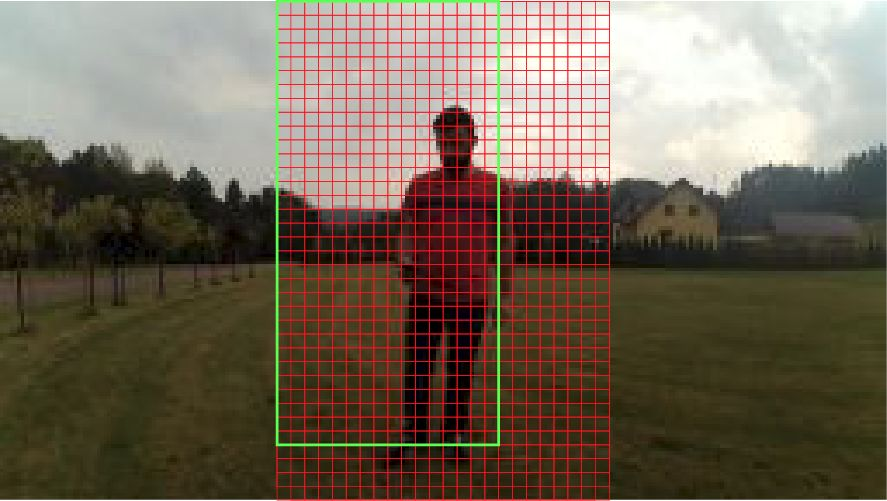
\includegraphics[width=15cm]{4_scaled_hog_example.jpg}
	\caption{Analiza obrazu o rozmiarach $144\times 256$}
	\label{fig:HOG_mesh}
\end{figure}
\newline
Jeśli algorytm będzie pracował na obszarze $144\times 96$, to zakładając stałe położenie komórek na obrazie (są to kwadraty $4\times4$ wydzielone czerwonymi liniami), powstanie łącznie $5\cdot9=45$ wektorów cech. Reszta obrazu zostaje zignorowana. Koordynaty centrum obszaru detekcji są określane na początku działania pojedynczej iteracji algorytmu i są natychmiastowo konwertowane do odpowiednich skal obrazu.

\subsection{Konwersja RGB do skali odcieni szarości}
Obraz wejściowy jest poddawany konwersji zgodnie ze wzorem \ref{eq:rgb2gray}. Używane są tu trzy równoległe mnożarki, a suma iloczynów jest zaokrąglana do 8 bitów (do postaci liczby całkowitej z zakresu 0-255).

\subsection{Skalowanie}
Kolejny etap to przeskalowanie obrazu wejściowego. Sama idea okazuje się być tym bardziej na miejscu, jeśli wziąć pod uwagę parametry kamery zamontowanej na dronie - w przypadku tego projektu jest to Xiaomi Yi, urządzenie do zastosowań sportowych, wyposażone w duży kąt widzenia - 155$^{\circ}$. W efekcie osoba oddalająca się od kamery bardzo szybko zmniejszy swoje wymiary na obrazie. Materiał $720\times 1280$ pikseli przeskalowano do 5 obrazów przy użyciu następujących skal:
\NumTabs{15}
\begin{itemize}
	\item \textbf{1:  2}\tab{:}\tab{$720\times 1280\rightarrow360\times 640$} pikseli
	\item \textbf{1:2.5}\tab{:}\tab{$720\times 1280\rightarrow288\times 512$} pikseli	
	\item \textbf{1:  3}\tab{:}\tab{$720\times 1280\rightarrow240\times 426$} pikseli
	\item \textbf{1:3.5}\tab{:}\tab{$720\times 1280\rightarrow205\times 365$} pikseli
	\item \textbf{1:  4}\tab{:}\tab{$720\times 1280\rightarrow180\times 320$} pikseli
\end{itemize}
Powyższe wartości pozwalają jednocześnie zachować prostotę implementacji (skale są reprezentowane w formacie U3.1) i wyraźnie określić odległość drona od postaci. 

Skalowanie przebiega w dość prosty sposób i polega na pomijaniu nieodpowiednich wierszy lub/i kolumn oryginalnego obrazu. Jeśli założyć, że:
\begin{itemize}
	\item $x_i$, $y_i$ - współrzędne obrazu wejściowego,
	\item $x_o$, $y_o$ - współrzędne obrazu wyjściowego (przeskalowanego),
	\item $s_c$ - skala do zastosowania w pionie oraz w poziomie,
\end{itemize}
to przypisanie wartości obrazu wejściowego nastąpi przy jednoczesnym spełnieniu obu poniższych warunków:
\begin{equation}
\label{eq:scaling}
\left.\begin{aligned} 
x_i&==\lfloor s_cx_o\rfloor \\ 
y_i&==\lfloor s_cy_o \rfloor
\end{aligned}\right.
\end{equation}
Po natrafieniu na odpowiedni piksel, oprócz przypisania jego wartości do wyjścia, wystawiony zostanie sygnał sterujący \textit{valid}, bardzo ważny dla dalszej części algorytmu.
Przykład dla kilku pierwszych wartości \textit{x\char`_o} jest widoczny w tabeli \ref{tab:scaling}.
\begin{table}[h]
	\centering
	\captionsetup{justification=centering,margin=1cm}
	\begin{tabular}{|P{2cm} |P{3cm} |P{2cm}|}	
		\hline
		\rowcolor{lightgray} $x_o$ & $x_is_c$ & $x_i$ \\ 
		1		& 2.5	& 2\\ 
		\hline
		2		& 5		& 5\\ 
		\hline
		3		& 7.5	& 7\\ 
		\hline
		4		& 10	& 10\\ 
		\hline		
	\end{tabular}
	\caption{Przykładowy przebieg skalowania dla $s_c=2.5$ wraz z przypisywanymi pikselami wejściowymi}
	\label{tab:scaling}
\end{table}

Działanie modułu opiera się na stworzeniu dwóch zestawów liczników dla każdej skali. Pierwszy zestawpozwala na zdeterminowanie indeksów piksela wejściowego ($x_i$, $y_i$) i został opisany w sekcji: \ref{sec:counter}. \newline
Drugi zestaw liczników działa zgodnie z poniższym schematem.
\begin{figure}[!h]
	\centering
	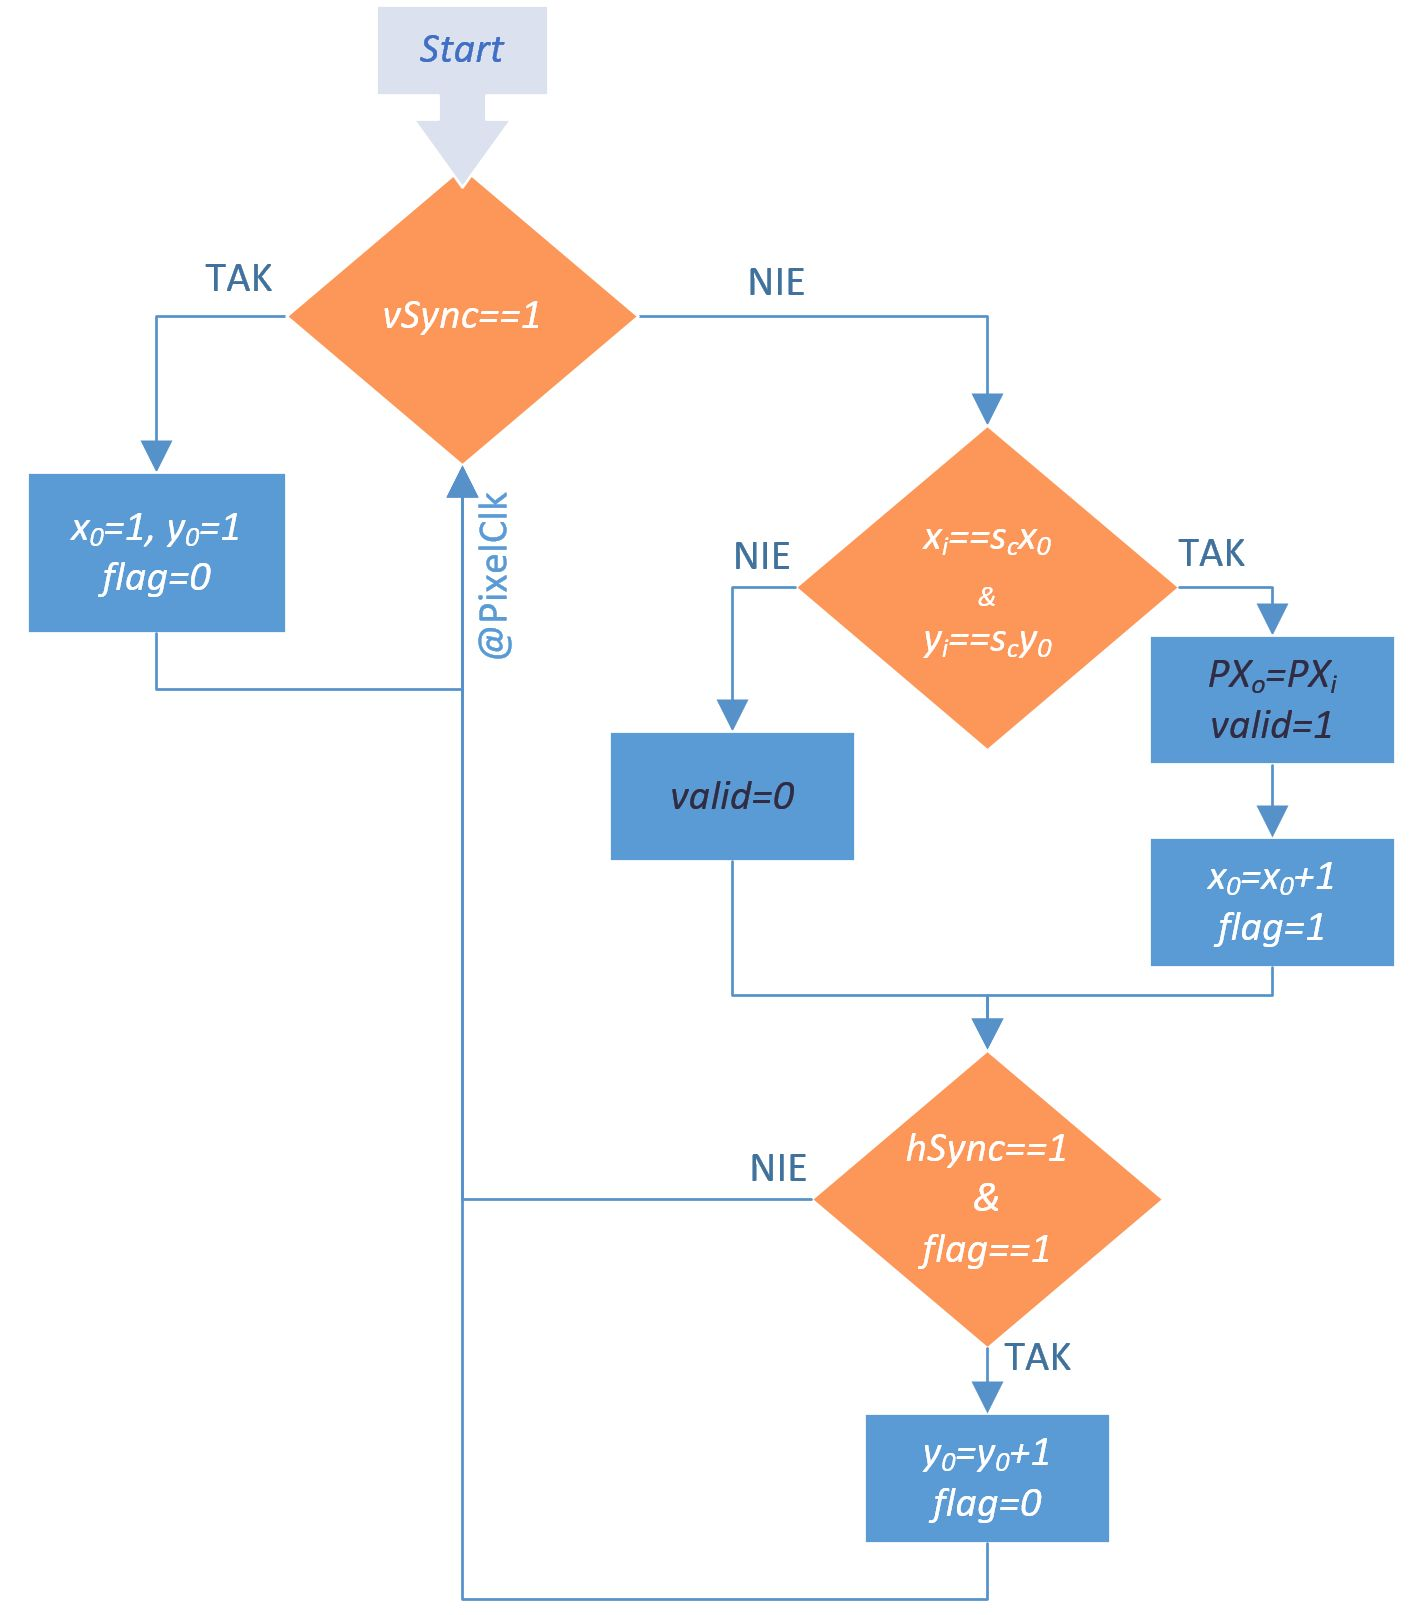
\includegraphics[width=11cm]{4_scaling.jpg}
	\caption{Schemat działania licznika skalującego}
	\label{fig:scaling_sch}
\end{figure}
Oznaczeniem \textit{@PixelClk} opisano proces oczekiwania na kolejne zbocze narastające zegara pikselowego. Gwarancją poprawnie przeprowadzonego procesu skalowania jest obecność sygnałów sterujących VGA - tylko wtedy następuje poprawny przyrost wartości liczników. Z kolei inicjalizacja (po lewej stronie diagramu) ma miejsce po otrzymaniu sygnału synchronizacji pionowej, zatem podłączony do układu sygnał wideo będzie skalowany już od pierwszej pełnej klatki.

\subsection{Obliczanie gradientów}
Nawet odpowiednio przeskalowane obrazy są zbyt duże, by przechowywać informację o ich gradientach. Nie ma jednak takiej potrzeby, jeśli postawi się na implementację algorytmu z maksymalizacją przetwarzania potokowego, opartego o sygnał aktywnego piksela \textit{valid} z modułu skalowania.

Implementacja gradientu pionowego jest nieco złożona, gdyż wymagane w pojedynczej operacji piksele leżą w kilku kolejnych liniach obrazu. Konieczne jest zapamiętanie dwóch ostatnich linii - zrealizowano to przy użyciu dwóch kolejek FIFO. Jedna z nich (oznaczona numerem \#1) rozpoczyna działanie już przy pierwszej linii obrazu i jej zadaniem jest przyjęcie aktualnych pikseli. Kolejka (\#2) przejmie je w kolejnej linii obrazu, gdy (\#1) pozbywając się starych pikseli „wymieni je” na te najnowsze - które wizualnie znajdują sie dokładnie pod nimi na obrazie. Logika została zaprojektowana w sposób pozwalający uzyskać jednoczesny dostęp do 3 kolejnych pikseli leżących w linii pionowej. Duża w tym zasługa specjalnego trybu modułu FIFO - First Word Fall Through (FWFT), dzięki któremu pierwsze dostępne słowo jest natychmiastowo wystawiane na wyjście, i tylko zdejmowane (zastępowane kolejnym) w odpowiedzi na wysoki stan sygnału odczytu.
Ostatecznie algorytm, będąc w linii $i$ ($i>1$), obliczy gradient pionowy dla piksela z linii $i-1$ - jak poniżej:
\begin{figure}[h]
	\centering
	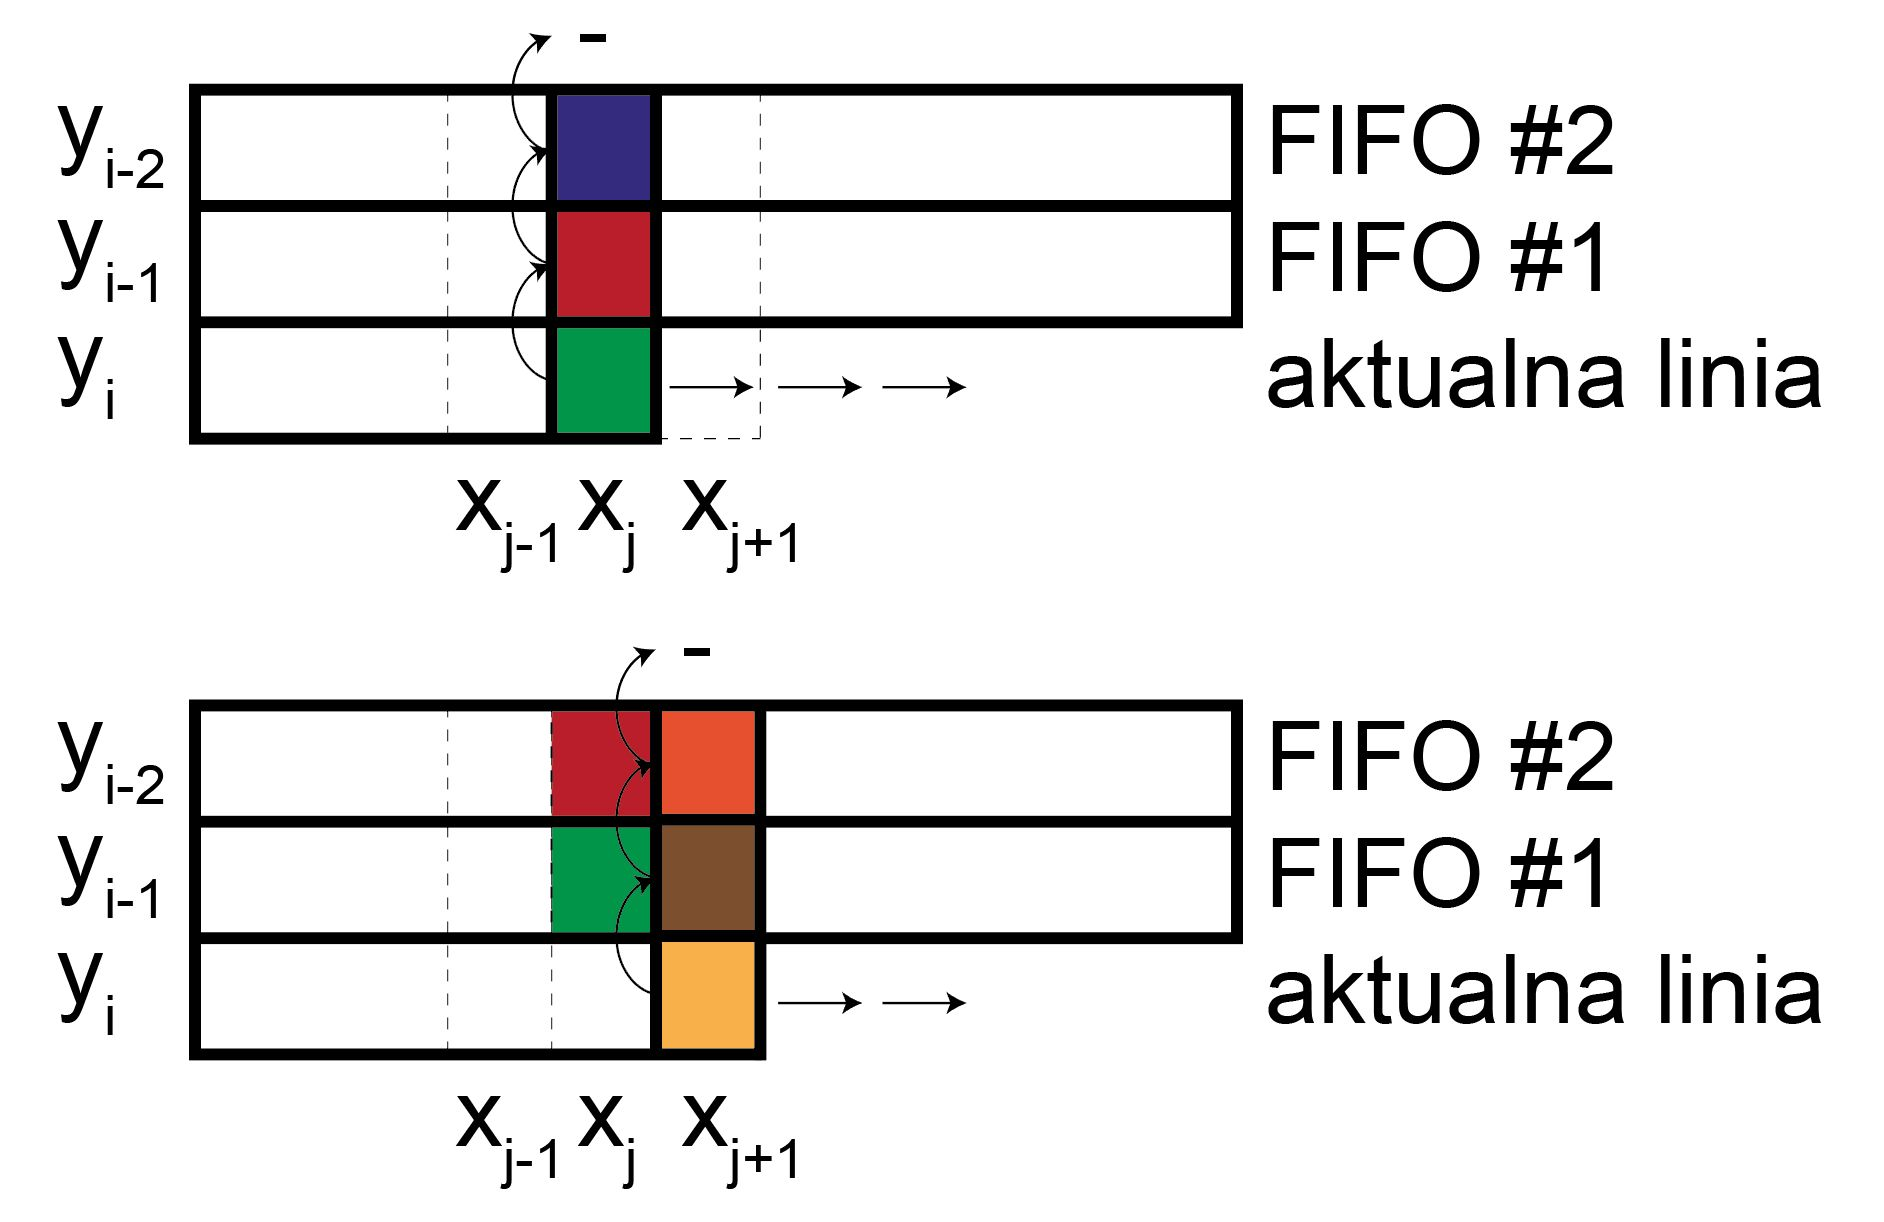
\includegraphics[width=11cm]{4_fifo_gradient.jpg}
	\caption{Schemat działania kolejek FIFO w procesie obliczania gradientu pionowego}
	\label{fig:fifo_gradient}
\end{figure}

Obliczanie gradientu poziomego nie nastręcza już tak wielu trudności - sąsiadujące ze sobą piksele pojawiają się tuż po sobie, jednak w tym wypadku zamiast aktualnych wykorzystywane są piksele wychodzące z FIFO \#1 i zapamiętywane w rejestrze przesuwnym. Oznacza to, że w chwili pojawienia się na wejściu do modułu nowego piksela ($i,j$), obliczony zostanie gradient poziomy piksela ($i-1,j-1$). Przez tę latencję potrzebne jest również nieznaczne opóźnienie gradientu pionowego, by obie wartości były zsynchronizowane i ustawione na wyjściu w tym samym momencie.

Sytuacje opisane powyżej dotyczą gradientów dla pikseli wewnątrz obrazu. Dla piksela znajdującego się na „początku” obrazu (lewa oraz górna krawędź), gradientem będzie dwukrotność różnicy pomiędzy nim a jedynym jego sąsiadem - w odpowiedniej osi. 

Piksele znajdujące się przy prawej i dolnej krawędzi ekranu wymagają innego podejścia. Poprzednie obliczenia były przeprowadzane w oparciu o sygnał aktywnego piksela ($valid$), którego zbocza były wykorzystywane do obliczeń gradientów aż do przedostatniego wiersza i kolumny obrazu ($i-1, j-1$). W tym przypadku, ich brak wymagał stworzenia logiki kontynuującej obliczenia i generującej wyjściowe sygnały aktywne. Brak dotychczasowych sygnałów \textit{valid} to również brak nowych danych dla kolejek FIFO, co skutkuje ich spodziewanym opróżnieniem krótko po odebraniu pełnej ramki obrazu. O ile poprzednio tempo obliczania gradientu było podyktowane pojawianiem się nowych pikseli i bezpośrednio powiązane z zastosowaną skalą, to w tym przypadku logika korzysta wyłącznie z opróżnianych kolejek FIFO, redukując odstęp pomiędzy wynikami do minimum (1 cykl zegara), co jest w zasadzie bez znaczenia dla dalszych obliczeń.

\subsection{Histogram gradientów}

Etapem następującym po uzyskaniu gradientu jest obliczenie wartości $arctg(\frac{g_y}{g_x})$. Wykorzystano tutaj blok IP CORDIC, który na wejściu spodziewa się wektora złożonego z licznika oraz mianownika o tych samych długościach, przy czym jego całkowita długość jest zaokrąglana do wielokrotności liczby 16. Gradienty uzyskane z poprzedniego modułu są zapisane w notacji S9.1, zatem wektor wejściowy musi mieć długość 32 - po 16 bitów na oba gradienty. Bardziej znaczące bity tych połówek zostały wypełnione zerami i nie mają znaczenia dla obliczeń. \newline 
Moduł będzie rozpoczynać obliczenia dla danych wejściowych tylko w przypadku, gdy policzone zostały oba gradienty (dwa niezależne sygnały \textit{valid\char`_x/y}), oraz gdy przynajmniej jeden z nich jest różny od zera ($\frac{0}{0}$ jest elementem nieoznaczonym, z którego nie sposób policzyć implementowaną funkcję). Opisane warunki \textit{valid\char`_x/y}, spięte odpowiednimi operatorami logicznymi, podłączono jako sygnał aktywny modułu. 

Otrzymane wartości należy następnie umieścić w dziewięciu 20-stopniowych przedziałach, co opisuje schemat \ref{fig:hog_gradient}. 
\begin{figure}[!ht]
	\centering
	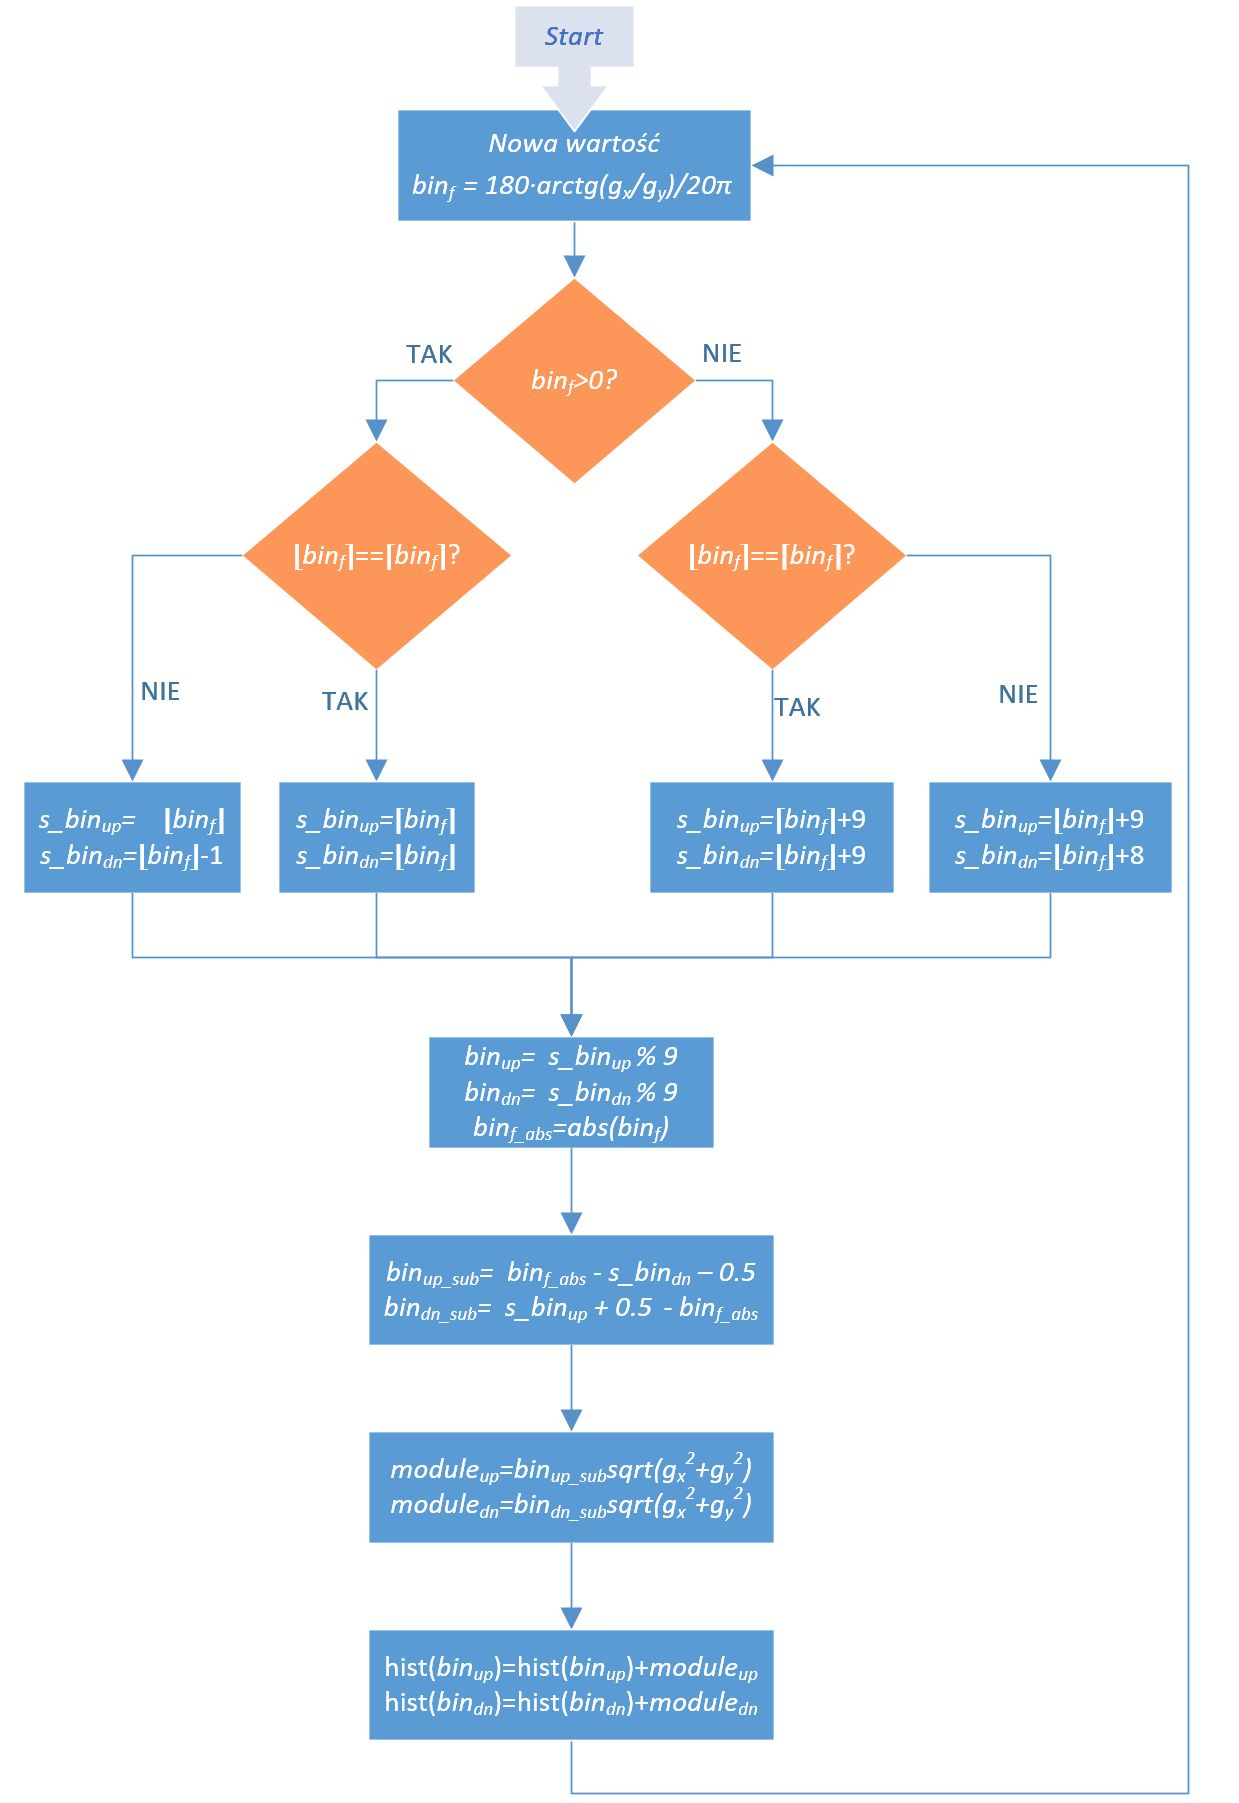
\includegraphics[width=12cm]{4_HOG_gradients.jpg}
	\caption{Schemat działania obliczeń prowadzących do utworzenia histogramu gradientów}
	\label{fig:hog_gradient}
\end{figure}
Pierwszym krokiem jest operacja mnożenia kątów podanych w radianach przez $\frac{180}{20\pi}$, która konwertuje je do liczb ułamkowych stanowiących wstępny przydział (niech będzie to $bin_f$).

Następnie, w zależności od położenia względem środka danego przedziału, wybierane są przedziały: górny i dolny w postaci liczb całkowitych: $s\_bin_{up}$ oraz $s\_bin_{dn}$. Ostateczne przedziały będą wymagać jednak normalizacji do postaci liczb z zakresu 0-8. Na ich podstawie tych wartości histogram powiększy dwa przedziały o interpolowane wartości modułu gradientów. 

Podstawową informacją wykorzystywaną w dalszej interpolacji jest odległość $abs(bin_f)$ od środków przedziałów $s\_bin_{up}$ oraz $s\_bin_{dn}$. Na tej podstawie obliczane są $module_{up}$ oraz $module_{dn}$ których suma jest równa modułowi gradientów.

Sam fragment logiki odpowiedzialny za obliczenie modułu został zrealizowany przy użyciu dwóch mnożarek dla obu gradientów, a sumę ich kwadratów następnie poddano pierwiastkowaniu blokiem CORDIC. Suma mnożeń jest wektorem U21.2, który poprzez dopisanie bitu '0' rozszerzono do U21.3. Zgodnie z dokumentacją modułu, wektor o tej długości jest traktowany przez CORDIC IP jako U1.23 - zatem jest wirtualnie przemnożony przez $2^{20}$. Wartość wyjściową należy później interpretować jako U11.13 (wirtualnie podzieloną przez $\sqrt{2^{20}}=2^{10}$). \newline
Ostateczne informacje - to jest dane o przedziałach i odpowiadające im części modułu zostały przekazane dalej, wraz z wygenerowanymi sygnałami aktywnymi.

Cały powyższy fragment podrozdziału skupiał się na operacjach związanych z pojedynczym pikselem. Teraz należy spojrzeć jednak z innej perspektywy, mianowicie na grupowanie pikseli w komórki, bloki i tworzenie wektorów cech na podstawie histogramu. \newline
Jak opisano we wstępie do rozdziału, najlepszy rezultat detekcji osiągnie się, realizując klasyfikację jak największej ilości wektorów cech wygenerowanych na obszarach z względnie niewielkim przesunięciem - jak zilustrowano to na \ref{fig:HOG_mesh}. Szybki przyrost zużycia zasobów układu ogranicza implementację do przetwarzania określonej ilości obszarów w sąsiedztwie miejsca podejrzewanego o obecność postaci.
Dane są bowiem zapisywane w pamięci BRAM. By nie marnować cennego miejsca w blokach BRAM, zdecydowano się zapisywać surowe histogramy, a nie gotowe wektory cech - wiedząc, że dalsza logika dokonując odczytu z tej pamięci, w odpowiedni sposób przekaże te informacje do klasyfikatora. Ostatecznie, pojedyncze okno detekcji $128\times 64$ to $32\cdot16=512$ histogramów, czyli $4608$ wartości. Wektor cech to aż $31\cdot15\cdot4\cdot9=16740$ wartości. Oszczędność wynikająca z zapisu pojedynczych histogramów pozwoli utworzyć znacznie więcej wektorów cech. Przykładowo, dla okna o wielkości $144\times 96$ należy zapisać $7776$ wartości. Pozwala to jednak wygenerować $9\cdot5=45$ wektorów cech - gdyby zaś wpisywać je do pamięci w gotowej formie, wymagałoby to aż $16740\cdot45=753300$ pozycji.

Pamięć RAM należy potraktować jako zbiór 9-elementowych histogramów ułożonych obok siebie. Przetwarzanie obrazu, rozumianego jako obiekt dwuwymiarowy, wymaga odpowiedniego mapowania tworzonych wartości do postaci jednowymiarowej, adresowej. Schemat \ref{fig:hog_histogram_scheme} przedstawia sposób pracy na ramce obrazu w kontekście zapisu do pamięci. Symbolem „$<=$” określa się przypisanie nieblokujące, które rzeczywisty efekt będzie miało dopiero na następnym zboczu narastającym zegara.
 
\begin{figure}[!ht]
	\centering
	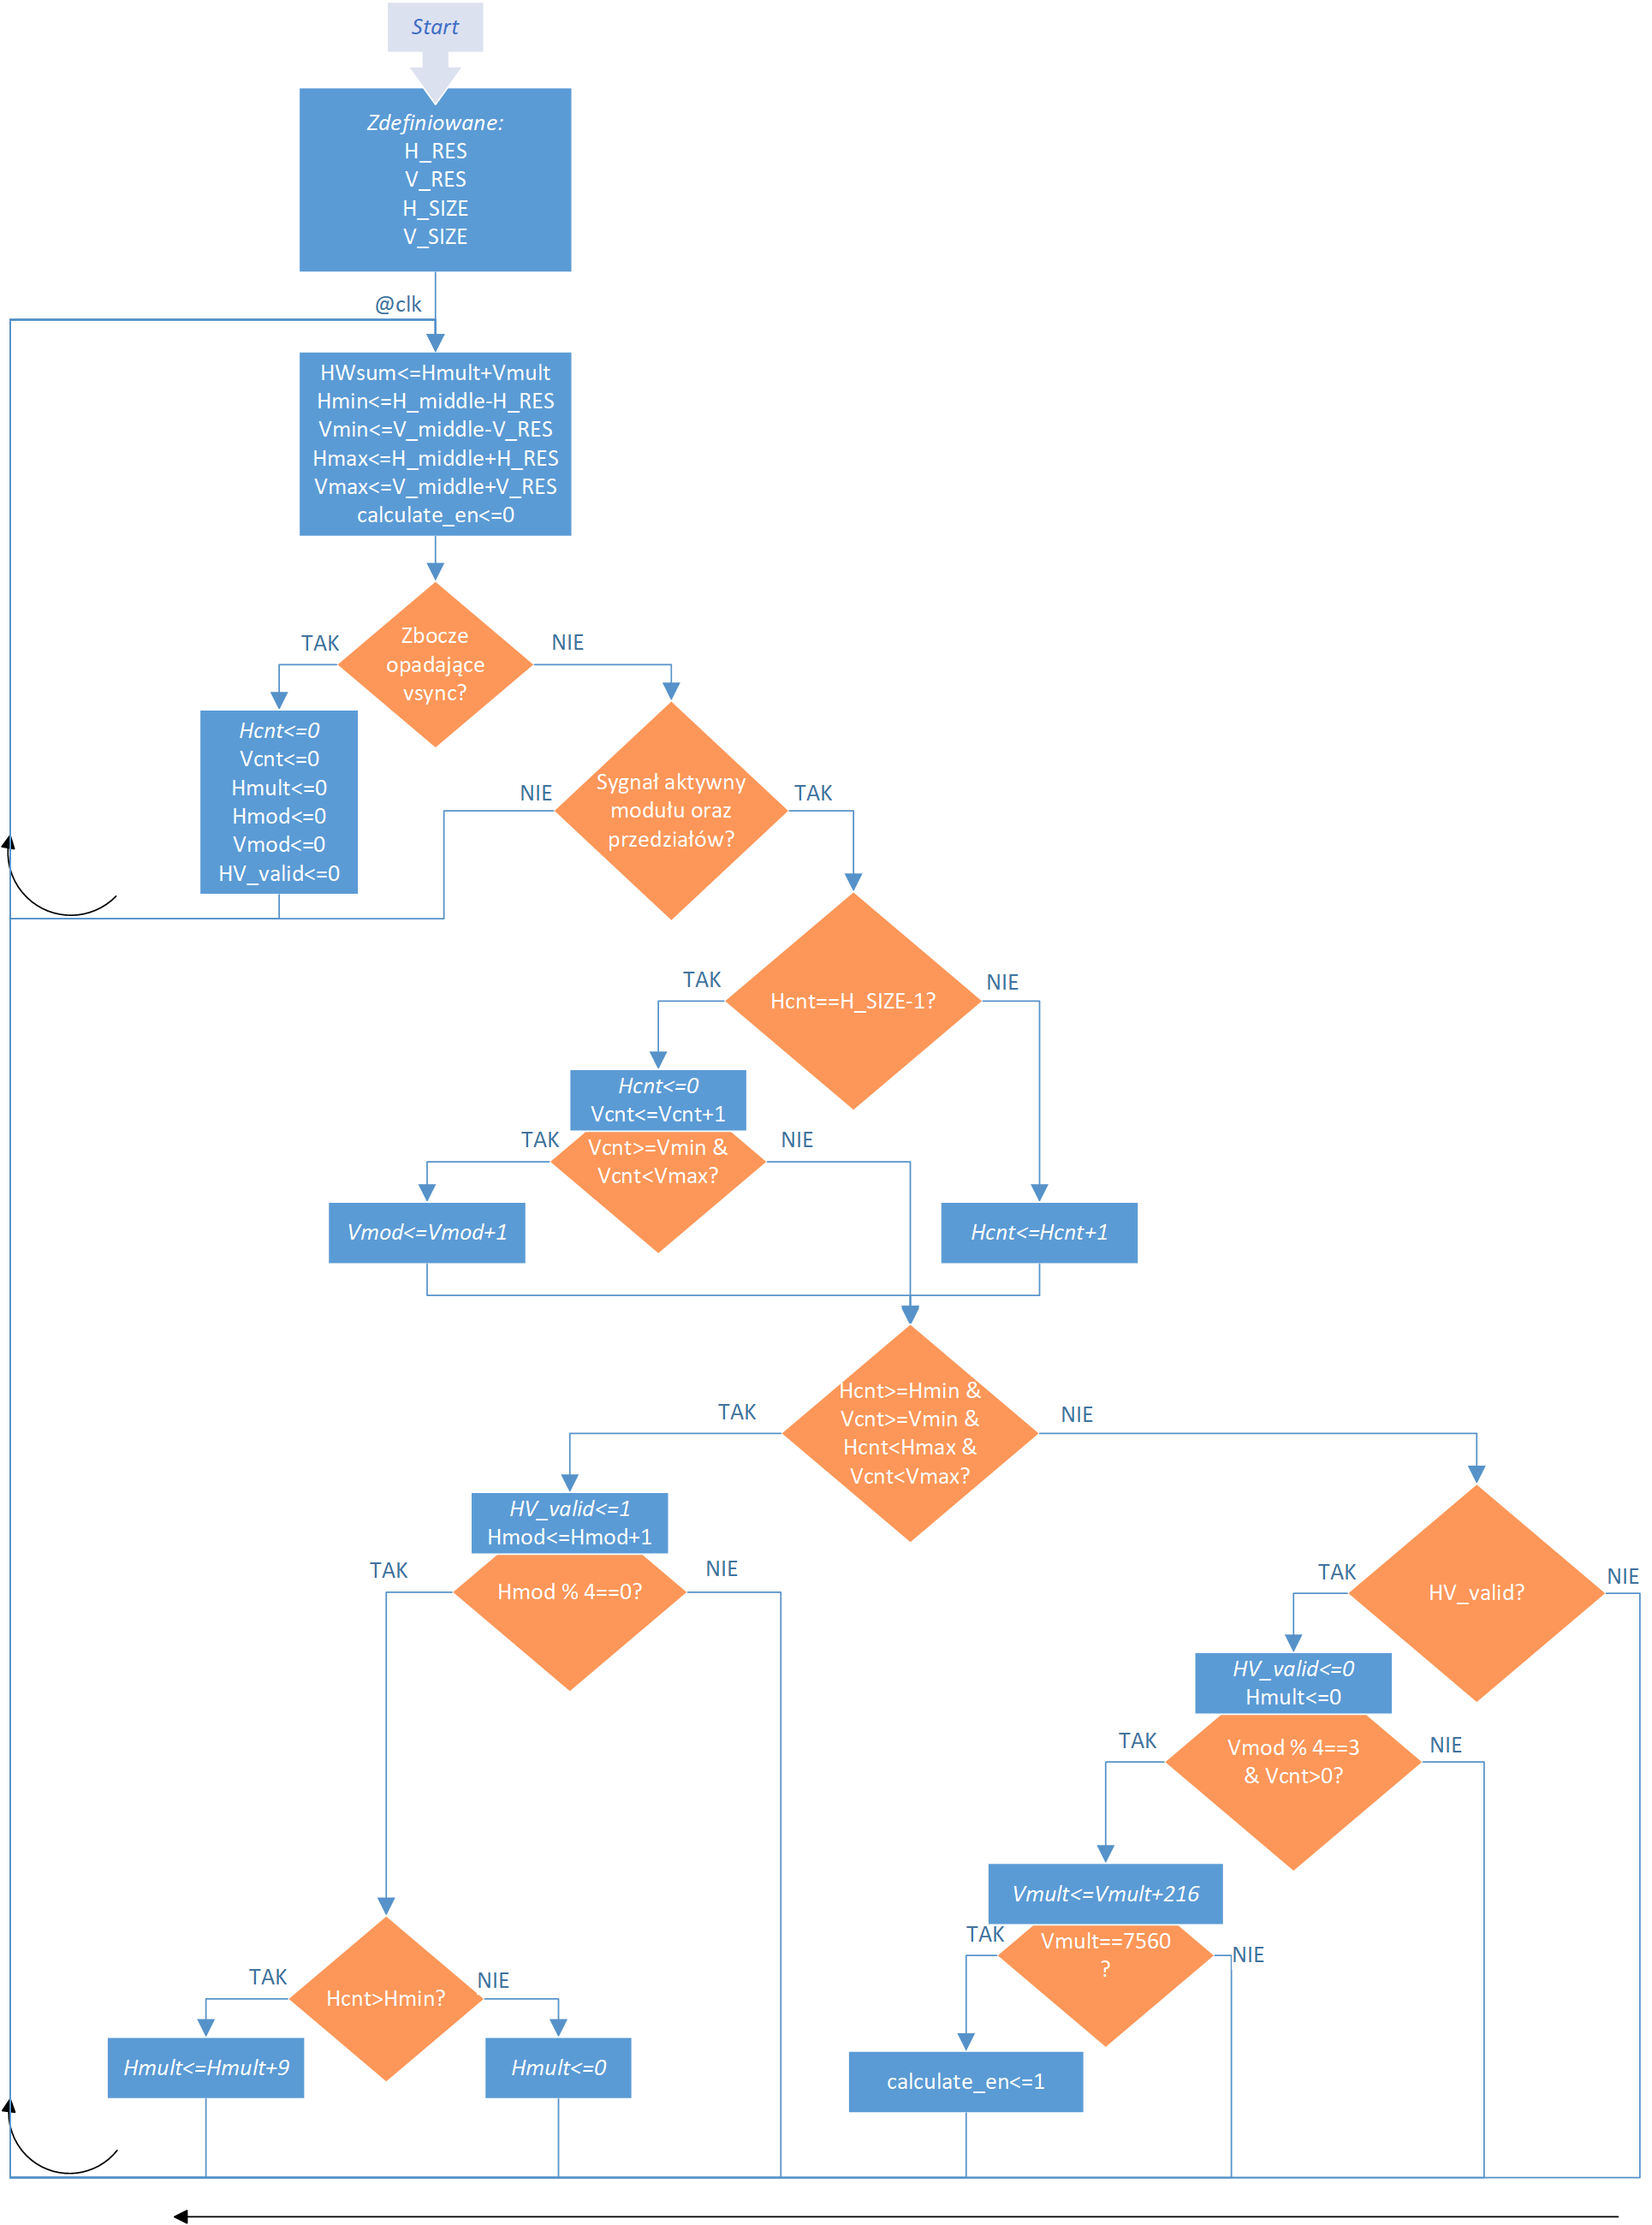
\includegraphics[width=16cm]{4_HOG_Histograms.png}
	\caption{Procedura wyboru adresu pamięci RAM w oparciu o pozycję aktualnego piksela}
	\label{fig:hog_histogram_scheme}
\end{figure} 
 
Określenie aktualnego położenia na obrazie jest możliwe dzięki zastosowaniu liczników, opierających swoje działanie na obecności sygnału aktywnego. Wykorzystano następujące parametry:
\begin{itemize}
	\item \textit{H\_SIZE}, \textit{V\_SIZE} - rozdzielczość obrazu przeskalowanego (indywidualnie dla każdej skali),
	\item \textit{H\_middle}, \textit{V\_middle} - koordynaty piksela środkowego, będącego w centrum analizowanego obszaru (w odniesieniu do odpowiedniej skali, dostarczone przed rozpoczęciem analizy pełnej klatki),
	\item \textit{H\_RES}, \textit{V\_RES} - wartości określające zasięg analizowanego obszaru - w odległości od piksela środkowego,
\end{itemize}
oraz zmienne:
\begin{itemize}
	\item \textit{Hcnt}, \textit{Vcnt} - zmienne inkrementowane odpowiednio do wartości maksymalnych \textit{H\_SIZE}, \textit{V\_SIZE} - pozwalają określić aktualne położenie na obrazie (i względem analizowanego obszaru),
	\item \textit{HV\_valid} - sygnał aktywny informujący o aktualnym położeniu wewnątrz analizowanego obszaru,
	\item \textit{Hmod}, \textit{Vmod} - liczniki modulo służące do rozdzielenia pikseli wchodzących w skład różnych histogramów (kwadratów o boku $4\times 4$),
	\item \textit{Hmult}, \textit{Vmult} - zmienne będące bazą adresową do zapisu aktualnego histogramu (horyzontalna zmienna powiększana o $9$, wertykalna o $9\cdot24$ - ilość histogramów w linii poziomej),
	\item \textit{calculate\_en} - sygnalizacja zakończonego procesu obliczania i zapisywania histogramów - możliwość rozpoczęcia klasyfikacji dla danej skali,.
\end{itemize}

Pamięć histogramu pracuje w trybie True Dual Port, umożliwiając jednoczesny dostęp do dwóch interpolowanych przedziałów aktualnego histogramu, $s\_bin_{up}$ oraz $s\_bin_{dn}$. Ich adresy są przedstawione równaniem:
\begin{equation}
\label{eq:adressing_hist}
\left.\begin{aligned} 
addr_{up}&=Hmult+Vmult+s\_bin_{up} \\ 
addr_{dn}&=Hmult+Vmult+s\_bin_{dn}
\end{aligned}\right.
\end{equation}
Zapis danych do pamięci histogramu jest realizowany, uprzednio odczytując aktualne wartości komórek i powiększając je odpowiednio o części modułu: $module_{up}$ oraz $module_{dn}$.



\subsection{Uczenie}
Uczenie to żmudny proces przetworzenia obrazów i ekstrakcji wektorów cech, na podstawie których powstanie płaszczyzna rozdzielająca próbki pozytywne od negatywnych. Przejście przez tak wielką ilość obrazów ma charakter jednorazowy, po którym będzie dysponować się parametrami umożliwiającymi klasyfikację. Z tego względu nie zdecydowano się na implementację modułu uczącego w układzie FPGA - tak ze względu na złożoność tego etapu, czas trwania procedury, jak i prawdopodobnie duży udział modułu w zużyciu zasobów logiki. 

Wybór padł na środowisko MATLAB, w którym zresztą wcześniej stworzono prototyp całego algorytmu (model programowy). Skrypt korzysta z plików tekstowych zawierających listy próbek do wczytania, które ostatecznie muszą być w rozmiarze $128\times 64$. Jak widać na ilustracji \ref{fig:HOG_image_examples}, wymiary próbek negatywnych mocno odbiegają od założonego wymiaru klasyfikowanego obrazu ($128\times 64$). Zdecydowano, iż w ich przypadku uczeniu poddany będzie obszar o wymiarach 128x64 wycięty ze środka oryginałów, jak i obraz przeskalowany oraz obcięty do wymiarów $128\times 64$. Na bazie tak przygotowanych próbek powstaje tablica deskryptorów oraz druga, która przechowuje odpowiadające im wartości klas (1 lub 0). Z obu tablic korzysta wbudowana funkcja \textit{svmtrain}, która zwraca strukturę ze współczynnikami. Z kolei \textit{svmclassify} jest w stanie odpowiednio zaklasyfikować obraz (a właściwie jego deskryptor). Tę funkcję użyto w procesie testowania niezależnego zestawu danych, by sprawdzić skuteczność wygenerowanych parametrów. Etap testowania jest dodatkowo przydatny - pozwala na bazie eksperymentów zdefiniować optymalny rozmiar komórki (kwadratu pikseli), na bazie których liczony jest pojedynczy histogram. Tabela \ref{tab:HOG_cell_size} prezentuje wyniki. Ekperyment przeprowadzono na komputerze wyposażonym w procesor Intela klasy i7, trzeciej generacji.
\newcolumntype{P}[1]{>{\centering\arraybackslash}p{#1}}
\begin{table}[h]
	\centering
	\captionsetup{justification=centering,margin=1cm}
	
	\begin{tabular}{|P{3cm} |P{3cm} |P{4.5cm}| P{3.5cm}|}	
		\hline
		\rowcolor{lightgray} Rozmiar komórki [px] & Ilość elementów wektora cech & Błąd klasyfikacji [\%]  & Czas trwania algorytmu [s] \\ 
		\lbrack$2\times $2\rbrack			& 70308		& 3.4069		& 52min 42s		\\ 
		\hline		
		\lbrack$4\times 4$\rbrack			& 16740 	& 2.3344		& 14min 08s		\\ 
		\hline
		\lbrack$8\times 8$\rbrack			& 3780		& 3.3438		& 05min 01s		\\ 
		\hline
		\lbrack$16\times 16$\rbrack			& 756		& 5.1735		& 02min 50s		\\ 
		\hline
	\end{tabular}
	
	\caption{Skuteczność algorytmu na zbiorze testowym w zależności od wielkości pojedynczej komórki}
	\label{tab:HOG_cell_size}
\end{table}
\newline
Okazuje się, że algorytm wykazuje największą skuteczność dla komórki o rozmiarze $4\times 4$ - zdecydowano się zatem na implementację algorytmu HOG w układzie FPGA właśnie w oparciu o tę wartość parametru. Szybkie obliczenia pokazują, że dla obrazu o wymiarach $128\times 64$ powstanie $32\times 16$ komórek, a idąc dalej, $31\times 15$ bloków po 4 histogramy po 9 wartości, czyli długość wektora cech będzie wynosić 16740. Oznacza to również, że po zakończonym procesie uczenia powstanie wektor współczynników o takiej długości.

Założeniem jest, by podczas pracy systemu wbudowanego nie ingerować we współczynniki, a raczej opierać się na pierwotnych wynikach uczenia. Dane te muszą być przechowane w odpowiedni sposób, by możliwy był do nich prosty i szybki dostęp. Postanowiono zapisać wektor w pamięci ROM inicjalizowanej plikami \textit{*.mem}, utworzonymi podczas wykonywania skryptu uczenia w MATLABie. Ręcznie dostosowany moduł pamięci posiada trzy niezależne sektory (w zakresie adresowania i długości danych), inicjalizowane następującymi informacjami: 

\begin{itemize}
	\item składniki skalujące - 16740 elementów wymaganych do przesunięcia każdego elementu wektora cech. Wartości w przedziale: $<-0.2616, -0.0527>$; precyzja zapisu: S0.11.
	\item czynniki skalujące - 16740 elementów do przemnożenia z powyższymi sumami. Wartości w przedziale: $<4.4207, 12.6310>$; precyzja zapisu: U4.8.
	\item współczynniki maszyny wektorów nośnych. Wartości w przedziale: $<   -0.0076, 0.0063>$; precyzja zapisu: S0.15 (oryginalnie w formacie S0.22, lecz 7 najstarszych bitów ma zawsze postać bitu znaku).
\end{itemize}

Dodatkowym współczynnikiem jest wartość przesunięcia gotowego wyniku o precyzji S0.40, jednak jest ona przechowywana w logice. 
Powyższa pamięć zajmuje aż 40 z wszystkich 140 bloków BRAM. Należy zauważyć, iż wymusza to współdzielenie pojedynczej instancji modułu we wszystkich procesach klasyfikacji. Z tego względu istotne jest stworzenie logiki synchronizującej początek przetwarzania wektorów cech ze wszytkich skal - opisuje to kolejna podsekcja.

\subsection{Klasyfikacja}
Etap klasyfikacji następuje bezpośrednio po obliczeniu wektorów cech. Odczytywane wartości pamięci ROM muszą być współdzielone pomiędzy obliczeniami przeprowadzanymi dla każdej ze skal obrazu, jednak w każdym przypadku tempo generowania histogramów nie jest jednakowe - proces przebiegnie szybciej dla większych obrazów (tam analizowany fragment obrazu pojawi się na wejściu wcześniej). O gotowości histogramów z odpowiedniej skali informuje indywidualny dla niej sygnał \textit{calculate\_en}. Dopiero w momencie otrzymania wszystkich sygnałów \textit{calculate\_en} (stan wysoki na wyjściu iloczynu logicznego) rozpoczynany jest właściwy proces klasyfikacji.

Moduł odpowiadający za sklasyfikowanie informacji pochodzących z pojedynczej skali zrealizowano w formie krótkiej maszyny stanu, na którą składają się następujące etapy:
\begin{itemize}
	\item inicjalizacja - oczekiwanie na sygnał \textit{full\_frame}, informujący o rozpoczęciu algorytmu na pełnej klatce obrazu
	\item czyszczenie pamięci przechowującej wektory cech z poprzednich uruchomień algorytmu - etap ten ma miejsce tuż po otrzymaniu sygnału \textit{full\_frame}, który pojawia się podczas stanu wysokiego synchronizacji pionowej; jest wykonywany na tyle szybko, by zdążyć przed pikselami wchodzącymi do modułu liczącego histogram.
	\item oczekiwanie na iloczyn sygnałów \textit{calculate\_en}; inicjalizacja zmiennych algorytmu
	\item właściwa klasyfikacja
\end{itemize}

O ile zapisane w pamięci ROM współczynniki mają postać wektora cech, tak pamięć RAM przechowuje nieuporządkowane fragmenty histogramów. Wymagało to stworzenia logiki, która skleja ze sobą dane z odpowiednich adresów pamięci, interpretując je w postać deskryptora. Opisuje to poniższy diagram.

\begin{figure}[!ht]
	\centering
	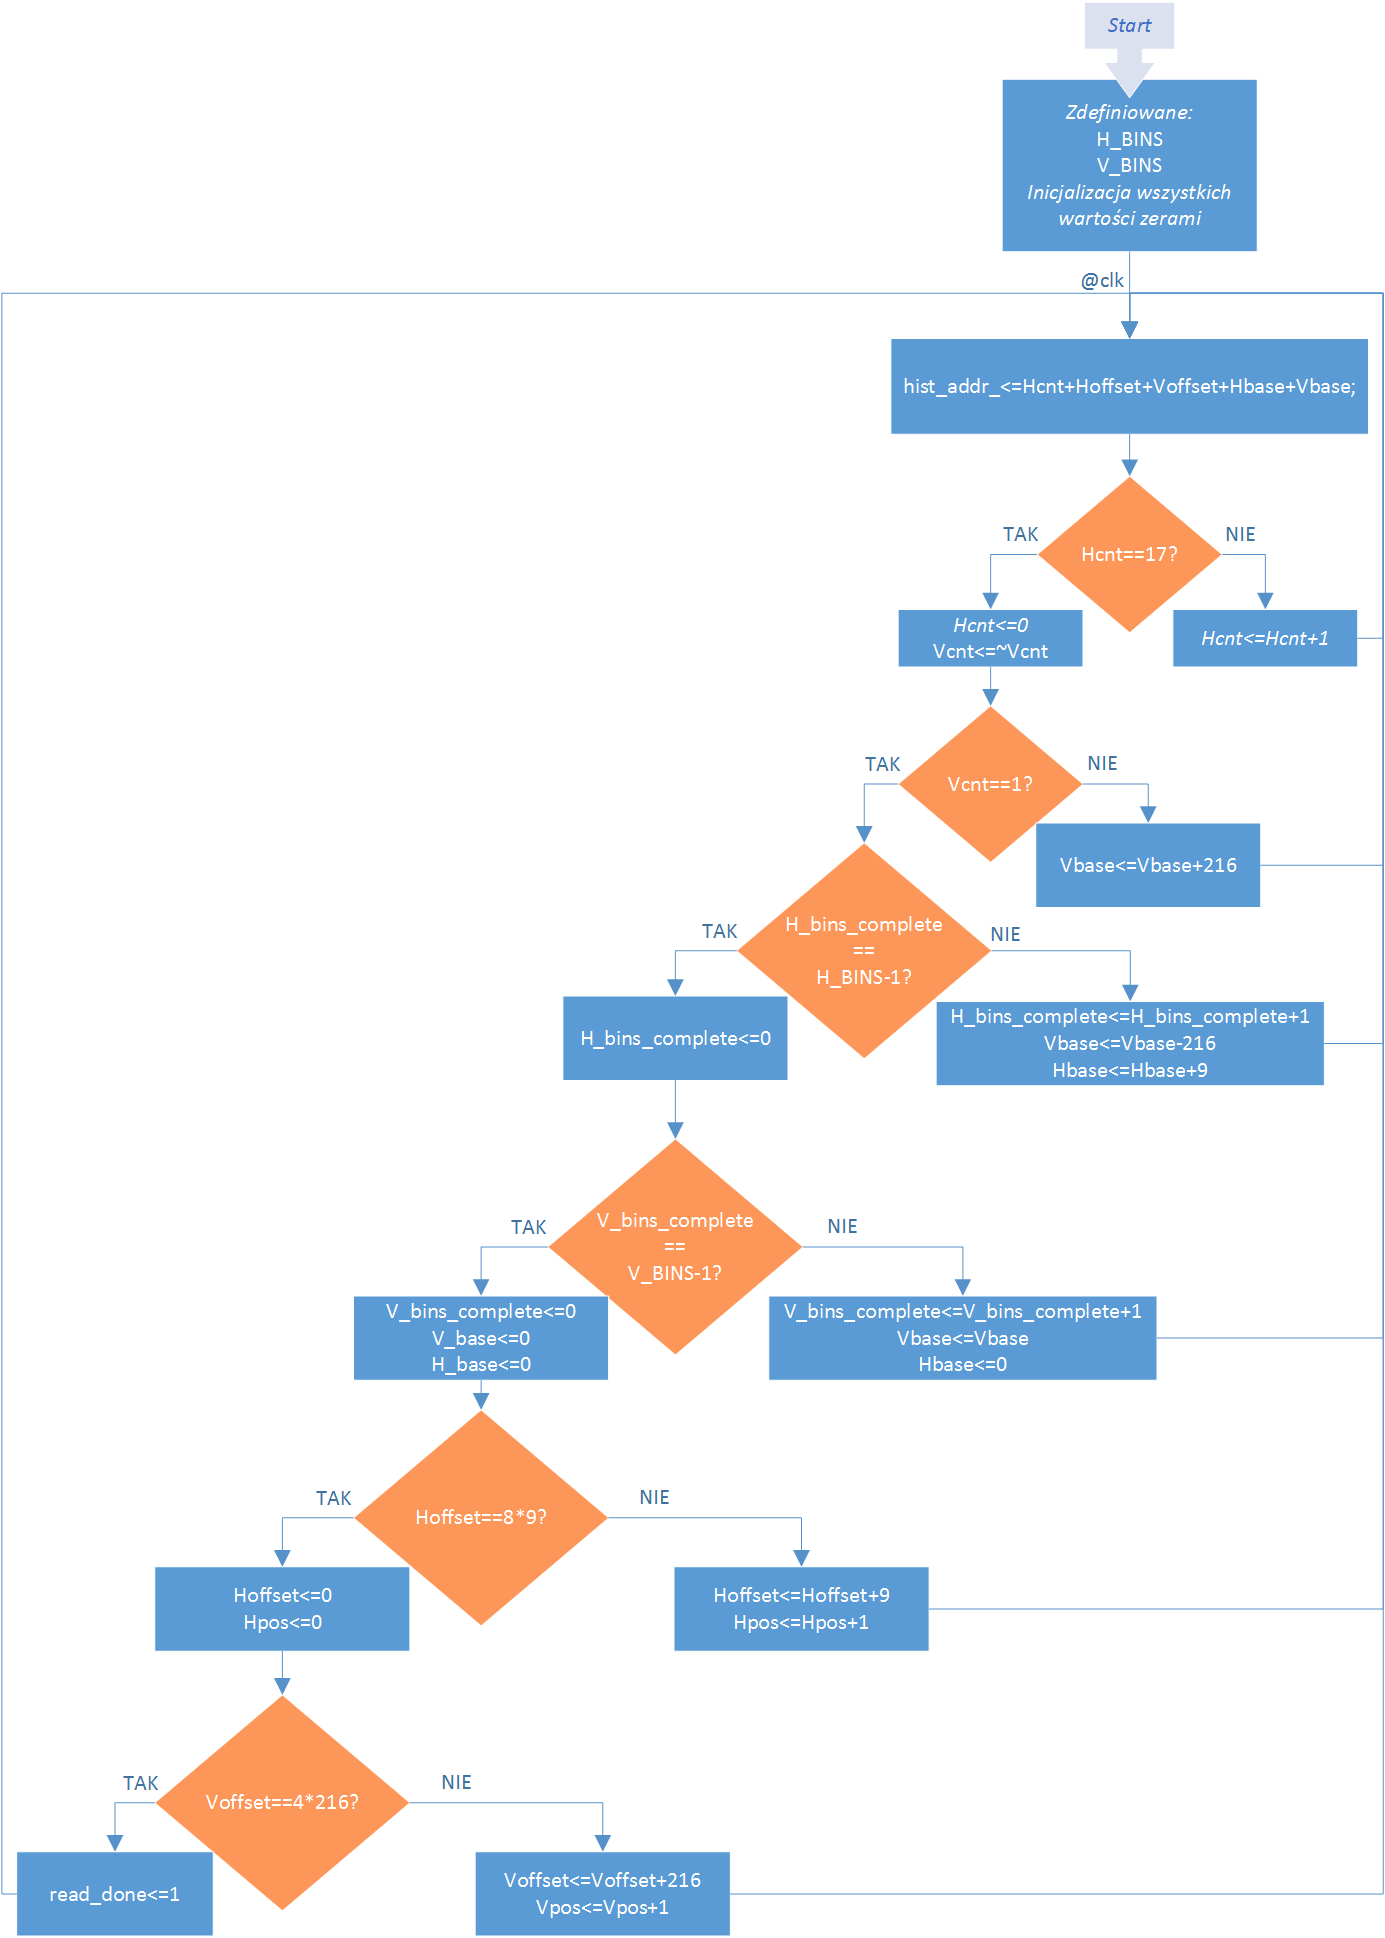
\includegraphics[width=16cm]{4_HOG_Features.png}
	\caption{Procedura wyboru adresu pamięci RAM w procesie odczytu kolejnych histogramów}
	\label{fig:hog_feature_histrogram_address}
\end{figure} 

Kolejnym etapem jest normalizacja bloków, która ze względu na prostszą realizację została umieszczona wewnątrz procesu klasyfikacji (chociaż właściwie idea bloków nie funkcjonowała we wcześniejszych modułach). Blokiem jest struktura 4 histogramów, czyli łącznie 36 wartości. Odczytane z pamięci RAM dane są podnoszone do kwadratu przez mnożarkę, a następnie inkrementowane. Suma 36 takich wartości jest pierwiastkowana i będzie stanowić mianownik w procesie normalizacji powiązanego bloku (zgodnie z równaniem \ref{eq:HOG_norm3}). Moduł pierwiastkujący działa potokowo, więc zwraca również wartość pierwiastkową z niepełnych sum - dlatego ważne jest wygenerowanie sygnału aktywnego w momencie zsumowania 36 elementów, a także zatrzaśnięcie poprawnej wartości pierwiastka na czas 36 dzieleń.

Normalizacja wymusza ponowne przejście przez odpowiednie dane pamięci RAM. Zastosowanie dwuportowego modułu pozwala na uzyskanie dostępu do uprzednio przetworzonych danych na drugim kanale, podczas gdy pierwszy port kontynuuje zwracanie informacji potrzebnych do obliczenia współczynników normalizacji dla kolejnych bloków. Poprawną kolejność danych na drugim porcie osiągnięto przez odpowiednie opóźnienie sygnału adresowego z portu pierwszego. 

Napływające potokowo dane z portu drugiego, podzielone przez odpowiedni współczynnik normalizacji, mają ustawioną flagę \textit{normalized\_valid}. Jej stan wysoki rozpoczyna  inkrementację adresu pamięci ROM przechowującej współczynniki przesunięć (\textit{shifts}). Każda z 16740 par zostanie do siebie dodana. Znormalizowane elementy wektora cech mają postać U11.13, zatem należało rozszerzyć wektor \textit{shifts}. 
\newline
Kolejnym krokiem jest wymnożenie każdej z sum przez czynnik skalujący, a następnie przez właściwy współczynnik maszyny wektorów nośnych. Aby to osiągnąć, należało ponownie i odpowiednio opóźnić linie adresowe uzyskujące dostęp do przestrzeni adresowej danych \textit{factors} oraz \textit{vectors}. Ostateczna szerokość pojedycznego elementu wynosi S0.40.

Docelowa wartość definiująca detekcję jest sumą wszystkich 16740 przetworzonych  elementów oraz jeszcze jednej stałej wyznaczonej na etapie uczenia, \textit{offset} równej $-0.6327$. \textit{Offset} stanowi wartość początkową sumy przy rozpoczęciu obliczeń nad kolejnym wektorem cech.
Ze względu na konieczność zapewnienia dobrej dokładności w procesie sumowania, wynik jest zapisywany w notacji S8.40, co wymaga rozszerzenia dodawanych elementów o 8 kopii najbardziej znaczącego bitu (będącego zresztą informacją o znaku).

\subsection{Przetwarzanie wyników}

Niezależnie od ilości przetwarzanych skal obrazu, całkowite zakończenie wszystkich klasyfikacji w systemie rozpocznie etap analizy wyników. Jest on dość prosty, gdyż zakłada jedynie porównanie najlepszych rezultatów ze wszystkich skal - w modułach klasyfikacji zaimplementowano logikę, która zapamiętuje swoje lokalne minima i parametry obszarów (w odpowiednich skalach), na podstawie których je osiągnięto. Skutkiem porównania jest wyłonienie skali z najlepszym wynikiem, a koordynaty tego obszaru zostają dostosowane do rozdzielczości natywnej i mogą być wykorzystane przez warstwę wyższą.



 